% Options for packages loaded elsewhere
% Options for packages loaded elsewhere
\PassOptionsToPackage{unicode}{hyperref}
\PassOptionsToPackage{hyphens}{url}
\PassOptionsToPackage{dvipsnames,svgnames,x11names}{xcolor}
%
\documentclass[
  english,
  review,
  number,
  sort,compress,
  authoryear,
  3p]{elsarticle}
\usepackage{xcolor}
\usepackage{amsmath,amssymb}
\setcounter{secnumdepth}{5}
\usepackage{iftex}
\ifPDFTeX
  \usepackage[T1]{fontenc}
  \usepackage[utf8]{inputenc}
  \usepackage{textcomp} % provide euro and other symbols
\else % if luatex or xetex
  \usepackage{unicode-math} % this also loads fontspec
  \defaultfontfeatures{Scale=MatchLowercase}
  \defaultfontfeatures[\rmfamily]{Ligatures=TeX,Scale=1}
\fi
\usepackage{lmodern}
\ifPDFTeX\else
  % xetex/luatex font selection
\fi
% Use upquote if available, for straight quotes in verbatim environments
\IfFileExists{upquote.sty}{\usepackage{upquote}}{}
\IfFileExists{microtype.sty}{% use microtype if available
  \usepackage[]{microtype}
  \UseMicrotypeSet[protrusion]{basicmath} % disable protrusion for tt fonts
}{}
\makeatletter
\@ifundefined{KOMAClassName}{% if non-KOMA class
  \IfFileExists{parskip.sty}{%
    \usepackage{parskip}
  }{% else
    \setlength{\parindent}{0pt}
    \setlength{\parskip}{6pt plus 2pt minus 1pt}}
}{% if KOMA class
  \KOMAoptions{parskip=half}}
\makeatother
% Make \paragraph and \subparagraph free-standing
\makeatletter
\ifx\paragraph\undefined\else
  \let\oldparagraph\paragraph
  \renewcommand{\paragraph}{
    \@ifstar
      \xxxParagraphStar
      \xxxParagraphNoStar
  }
  \newcommand{\xxxParagraphStar}[1]{\oldparagraph*{#1}\mbox{}}
  \newcommand{\xxxParagraphNoStar}[1]{\oldparagraph{#1}\mbox{}}
\fi
\ifx\subparagraph\undefined\else
  \let\oldsubparagraph\subparagraph
  \renewcommand{\subparagraph}{
    \@ifstar
      \xxxSubParagraphStar
      \xxxSubParagraphNoStar
  }
  \newcommand{\xxxSubParagraphStar}[1]{\oldsubparagraph*{#1}\mbox{}}
  \newcommand{\xxxSubParagraphNoStar}[1]{\oldsubparagraph{#1}\mbox{}}
\fi
\makeatother


\usepackage{longtable,booktabs,array}
\usepackage{calc} % for calculating minipage widths
% Correct order of tables after \paragraph or \subparagraph
\usepackage{etoolbox}
\makeatletter
\patchcmd\longtable{\par}{\if@noskipsec\mbox{}\fi\par}{}{}
\makeatother
% Allow footnotes in longtable head/foot
\IfFileExists{footnotehyper.sty}{\usepackage{footnotehyper}}{\usepackage{footnote}}
\makesavenoteenv{longtable}
\usepackage{graphicx}
\makeatletter
\newsavebox\pandoc@box
\newcommand*\pandocbounded[1]{% scales image to fit in text height/width
  \sbox\pandoc@box{#1}%
  \Gscale@div\@tempa{\textheight}{\dimexpr\ht\pandoc@box+\dp\pandoc@box\relax}%
  \Gscale@div\@tempb{\linewidth}{\wd\pandoc@box}%
  \ifdim\@tempb\p@<\@tempa\p@\let\@tempa\@tempb\fi% select the smaller of both
  \ifdim\@tempa\p@<\p@\scalebox{\@tempa}{\usebox\pandoc@box}%
  \else\usebox{\pandoc@box}%
  \fi%
}
% Set default figure placement to htbp
\def\fps@figure{htbp}
\makeatother



\ifLuaTeX
\usepackage[bidi=basic]{babel}
\else
\usepackage[bidi=default]{babel}
\fi
% get rid of language-specific shorthands (see #6817):
\let\LanguageShortHands\languageshorthands
\def\languageshorthands#1{}
\ifLuaTeX
  \usepackage[english]{selnolig} % disable illegal ligatures
\fi


\setlength{\emergencystretch}{3em} % prevent overfull lines

\providecommand{\tightlist}{%
  \setlength{\itemsep}{0pt}\setlength{\parskip}{0pt}}



 
\usepackage[]{natbib}
\bibliographystyle{elsarticle-harv}


\usepackage{setspace}
\doublespacing
\usepackage{lineno}
\linenumbers
\makeatletter
\@ifpackageloaded{caption}{}{\usepackage{caption}}
\AtBeginDocument{%
\ifdefined\contentsname
  \renewcommand*\contentsname{Table of contents}
\else
  \newcommand\contentsname{Table of contents}
\fi
\ifdefined\listfigurename
  \renewcommand*\listfigurename{List of Figures}
\else
  \newcommand\listfigurename{List of Figures}
\fi
\ifdefined\listtablename
  \renewcommand*\listtablename{List of Tables}
\else
  \newcommand\listtablename{List of Tables}
\fi
\ifdefined\figurename
  \renewcommand*\figurename{Figure}
\else
  \newcommand\figurename{Figure}
\fi
\ifdefined\tablename
  \renewcommand*\tablename{Table}
\else
  \newcommand\tablename{Table}
\fi
}
\@ifpackageloaded{float}{}{\usepackage{float}}
\floatstyle{ruled}
\@ifundefined{c@chapter}{\newfloat{codelisting}{h}{lop}}{\newfloat{codelisting}{h}{lop}[chapter]}
\floatname{codelisting}{Listing}
\newcommand*\listoflistings{\listof{codelisting}{List of Listings}}
\makeatother
\makeatletter
\makeatother
\makeatletter
\@ifpackageloaded{caption}{}{\usepackage{caption}}
\@ifpackageloaded{subcaption}{}{\usepackage{subcaption}}
\makeatother
\journal{Computers and Electronics in Agriculture}
\usepackage{bookmark}
\IfFileExists{xurl.sty}{\usepackage{xurl}}{} % add URL line breaks if available
\urlstyle{same}
\hypersetup{
  pdftitle={Explainable machine learning for wheat above-ground biomass estimation under spatial cross-validation: sensor contributions and exploratory harvest forecasting},
  pdfauthor={Francisco Zambrano; Abel Herrera; Mauricio Molina-Rocco},
  pdflang={en},
  pdfkeywords={above-ground
biomass, Sentinel‑1, Sentinel‑2, PlanetScope, soil moisture, machine
learning, precision agriculture},
  colorlinks=true,
  linkcolor={blue},
  filecolor={Maroon},
  citecolor={Blue},
  urlcolor={Blue},
  pdfcreator={LaTeX via pandoc}}


\setlength{\parindent}{6pt}
\begin{document}

\begin{frontmatter}
\title{Explainable machine learning for wheat above-ground biomass
estimation under spatial cross-validation: sensor contributions and
exploratory harvest forecasting}
\author[1]{Francisco Zambrano%
%
}

\author[2]{Abel Herrera%
%
}

\author[3]{Mauricio Molina-Rocco%
%
}


\affiliation[1]{organization={Facultad de Economía, Negocios y Gobierno,
Universidad San Sebastián, Santiago, Chile},,postcodesep={}}
\affiliation[2]{organization={Hemera Centro de Observación de la Tierra,
Facultad de Ciencias, Ingeniería y Tecnología; Universidad Mayor,
Santiago, Chile},,postcodesep={}}
\affiliation[3]{organization={Laboratorio de Suelos y Sostenibilidad.
Departamento de Acuicultura y Recursos Agroalimentarios, Universidad de
Los Lagos, Osorno, 5311157, Chile},,postcodesep={}}

\cortext[cor1]{Corresponding author}



        
\begin{abstract}
Global food security faces increasing challenges under climate change,
making accurate monitoring of wheat (\emph{Triticum aestivum}) critical.
This study presents an explainable machine learning (ML) framework to
estimate in-season wheat above-ground biomass (AGB) and to explore
harvest forecasting one to four months ahead, integrating in-situ
weather and soil moisture data with Sentinel-1, Sentinel-2, and
PlanetScope imagery across four Mediterranean wheat field-seasons
(2020--2023) in central Chile. We evaluated 41 models---40
recipe-algorithm combinations spanning eight sensor-combination recipes
and five ML algorithms (Random Forest {[}RF{]}, XGBoost, GLMnet, bagMLP,
and KNN), plus a stacked ensemble---and obtained a preliminary,
exploratory assessment of their spatial transferability with a
leave-one-site-out cross-validation (LOSO-CV) scheme across the four
site-seasons, with model transparency assessed via the DALEX framework.

For in-season estimation (stage 1), the best LOSO-CV configuration (RF
using only PlanetScope predictors, \emph{rec7}) reached R²=0.78
(RMSE=7.87 t/ha, MAE=5.90 t/ha). A sensor-ablation analysis showed that
Sentinel-2 reduced RMSE by 23.4\% relative to a weather-only baseline,
Sentinel-1 added essentially no further skill (+0.5\%), and PlanetScope
contributed a further 5.7\% reduction. DALEX analysis of the stacked
ensemble identified a Sentinel-2 SWIR-related chlorophyll index
(S2\textsubscript{SWIR12}-MCARI), two PlanetScope band/index predictors,
a cumulative Sentinel-2 red-edge index, and the Sentinel-1 VH/VV
backscatter ratio as the leading, comparably important predictors,
spanning optical, SAR, and accumulated-thermal-time variables. As a
secondary, exploratory objective, the same LOSO-CV framework was applied
to a self-consistency analysis of harvest-AGB forecasting one to four
months ahead, using the stage 1 model's own spatial predictions as the
target in the absence of independent harvest-date ground truth;
self-consistency (RF, all predictors) was modest and decayed sharply
with lead time (R² from 0.46 at one month to 0.10 at four months; RMSE
from 4.5 to 6.5 t/ha), underscoring the need for both independent
harvest-date measurements and larger multi-site networks to properly
evaluate multi-month forecasting. This multi-sensor, cloud-resilient
framework provides a promising, explainable basis for in-season AGB
monitoring in Mediterranean wheat systems, although the four-site-season
LOSO-CV evaluation should be read as a preliminary sensitivity analysis
of spatial transferability rather than definitive proof of
generalizability (see Discussion).
\end{abstract}





\begin{keyword}
    above-ground
biomass \sep Sentinel‑1 \sep Sentinel‑2 \sep PlanetScope \sep soil
moisture \sep machine learning \sep 
    precision agriculture
\end{keyword}
\end{frontmatter}
    

\section{Introduction}\label{introduction}

As the world population is projected to reach 9.8 billion by 2050
\citep{UN2024}, food security is expected to face significant challenges
\citep{Bahar2020}, which are further intensified by climate change
\citep{Chen2025}. Wheat (\emph{Triticum aestivum}) is the most consumed
crop worldwide, and its production is key for food security
\citep{FAO2025}. Furthermore, droughts significantly impact agriculture,
as evidenced by the decrease in crop yield
\citep{Santini2022, Naumann2021, Mishra2015}. In fact, global wheat
production could drop by 13\% by mid-century under climate change
\citep{Pequeno2024}. Quantifying above-ground biomass (AGB) is of utmost
importance since it allows us to monitor and optimize agricultural
processes \citep{Dietz2021}. Proxies of vegetation productivity derived
from vegetation indices can help monitor and predict the impact of
drought at a regional scale
\citep{Zambrano2021, Zambrano2018, Zambrano2016}. However, on a farm
level, we must quantify this impact using crop yield as a productivity
metric, which can aid in determining the economic impact of seasonal
variations in crop yield. Generally, the estimation and monitoring of
agricultural production is made by using three methods: i) crop growth
models \citep{Lobell2010, Wang2023}, ii) surveys \citep{Gardner1980},
and iii) in-situ measurements. The models help predict how crops will
grow, yield, and produce under different environmental and management
conditions, which is useful for forecasting food supply and
understanding how climate change and policy decisions affect global
agriculture, but the downside is that they require many different
variables to obtain meaningful results. The objective of the surveys is
to collect timely and reliable data from the agricultural sector in
order to carry out statistical studies of crops, but it provides
summaries at administrative units (e.g., states, districts)
\citep{Gardner1980}. Additionally, field measurements provide reliable
data---known as the ground truth---that can be used for comparison with
models and surveys; however, this process is costly and time-consuming.

The use of empirical models that are based solely on remote sensing
sources has become a straightforward option for the estimation of crop
yield, especially for cereals \citep{Lischeid2022}. There are multiple
remote sensing methods to estimate AGB, among which the methods based on
multispectral imaging \citep{Marshall2022, Segarra2022}, Synthetic
Aperture Radar (SAR) \citep{Hu2024, Chao2019}, LiDAR (Light Detection
and Ranging) \citep{Bates2021}, hyperspectral \citep{Yue2021}, or
combination of them \citep{Li2024, David2022, Wang2016}, stand out,
offering promising results. Estimation methods based on SAR data focus
on the measurement of the structure of the crop, soil moisture, and
their temporal variations. An advantage of this technique is that it can
penetrate the cloud cover, allowing a constant measurement in the study
area; its disadvantage is the angle of observation to the crop and the
speckle noise inherent to the signal
\citep{Lopes1990, Maghsoudi2012, Moran1997}. Estimation methods based on
LiDAR and hyperspectral data focus on the measurement of the crop
structure and phenological monitoring of the crop
\citep{Brovkina2017, Luo2017, Wang2016}. Its main disadvantage is the
high cost of implementation, which limits its proliferation. Another
common approach is the use of spectral indices (e.g., NDVI, EVI, etc.)
derived from optical sensors such as Sentinel-2 \citep{David2022} for
specific dates. Furthermore, the use of accumulated spectral indices
\citep{PeroniVenancio2020} over the growing season has shown
improvements in estimating biomass/yield compared with using indices
just for specific dates. The main advantage is its simplicity and strong
correlation with the observed biomass. Currently, the research about
estimating biomass is moving forward integrating Sentinel 1 \& 2
\citep{Uribeetxebarria2023}, LiDAR, hyperspectral, and Landsat missions
\citep{Zhang2023, He2018}, which aids in better monitoring of the crop's
growth stages \citep{Shen2023}.

Effective machine learning (ML) methods, along with remote sensing data,
are increasingly used to estimate the AGB in various cereals, including
wheat. In Southern Brazil, \citep{AtkinsonAmorim2022} collected images
from unmanned aerial vehicles (UAV) and used random forest, support
vector regressions, and neural networks to estimate AGB in wheat. Their
results reached a R² of 0.90 and a root mean square error (RMSE) of 0.83
t/ha. In another study, \citep{Liu2024} used spectral data obtained from
UAV, phenological information, and multiple machine learning algorithms
to estimate AGB on wheat, having results of an R² ranging from 0.84 to
0.91 and an RMSE of 1.69 to 2.11 t/ha. Considering another approach,
\citep{Marshall2022} used hyperspectral and Sentinel-2 data and applied
random forest and partial least squares to estimate wheat AGB on
different stages of the crop. Their results achieve an R²=0.81 and
RMSE=3.7 t/ha with the random forest model. Further, for different types
of grass cover, Sentinel-1 has been tested to estimate AGB with varied
results \citep{David2022, Li2024, Nuthammachot2022}. The benefits of SAR
Sentinel-1 are that it can gather dependable data even on cloudy days,
which is not possible with optical sensors like Sentinel-2 and Landsat.
Additionally, Sentinel-1's backscatter is closely linked to the
dielectric constant, making it a proxy of soil moisture
\citep{Fan2025, Zhu2024}, and, therefore, the amount of water crops can
absorb from the soil, which affects their growth. Thus, it is worthwhile
to explore its usefulness for AGB prediction.

Here, we aim to develop and evaluate an explainable ML framework for
estimating wheat AGB during the growing season from multi-sensor remote
sensing (Sentinel-1, Sentinel-2, and PlanetScope) and in-situ weather
and soil moisture data, and to obtain a preliminary, exploratory
assessment of its spatial transferability under a leave-one-site-out
cross-validation (LOSO-CV) scheme across four Mediterranean wheat
field-seasons. As a secondary, exploratory objective, we evaluate
whether the same predictors and modeling framework can reproduce, from
earlier-season covariates, the framework's own spatial AGB predictions
at harvest one to four months in advance. We defined three specific
objectives: i) derive predictors from weather, soil moisture,
Sentinel-1, Sentinel-2, and PlanetScope data; ii) apply ML algorithms
together with explainable-AI techniques to estimate the spatiotemporal
variation of wheat AGB through the growing season and identify which
sensors and variables drive model performance; and iii) explore the
feasibility of forecasting AGB at harvest at four lead times (one to
four months before harvest) using the same modeling and LOSO-CV
validation framework.

\section{Materials and Methods}\label{materials-and-methods}

\subsection{Study Area}\label{study-area}

The study was conducted during the 2020--2023 growing seasons
(June--January) across four wheat field sites (\emph{Triticum}
\emph{aestivum}) located in central Chile: i) La Cancha in the
Metropolitan region, ii) Hidango in the O'Higgins region (two different
fields in two seasons), and iii) Villa Baviera in the Maule region.
Sampling took place in delineated fields at each site
(Figure~\ref{fig-1}). In Hidango, separate fields were established for
the 2021-2022 and 2022-2023 seasons; in Villa Baviera and La Cancha,
sampling occurred during the 2020-2021 and 2022-2023 seasons,
respectively. To capture spatial variability and ensure
representativeness, sampling points were randomly selected and evenly
distributed: five in La Cancha, Villa Baviera, and the northern Hidango
field (2021--2022 season); and six in the southern Hidango field
(2022--2023 season) (Figure~\ref{fig-1}).

\begin{figure}

\centering{


\includegraphics[width=1\linewidth,height=\textheight,keepaspectratio]{../output/figs/area_estudio_v2.png}

}

\caption{\label{fig-1}\textbf{Study Area.} The map on the left panel
shows the location of the sites in Central Chile. The remaining panels
illustrate the field boundaries and sampling points for each site. In
Hidango, the northern field is from the 2021--2022 season, and the
southern one from 2022--2023.}

\end{figure}%

A variety of spring wheat was planted in Villa Baviera (Llareta-INIA;
\citep{Garrido2013}), while the other sites had winter wheat
(Irafen-INIA and Pantera-INIA; \citep{DelPozo2023}). Spring wheat is
typically sown in late winter or early spring and harvested within the
same year, whereas winter wheat is sown in autumn, requires
vernalization, and is harvested the following summer
\citep{Liu2025, Zhao2022}. According to the FAO--UNESCO Soil Map of the
World \citep{FAO2014}; La Cancha is characterized by shallow,
fine-textured Regosols on nearly flat terrain; Hidango presents
fine-textured Luvisols on gently undulating landscapes; and Villa
Baviera features deep, well-structured Nitisols on slightly sloped land.
The climate in these regions is Mediterranean with winter rainfall (Csb)
under the Köppen--Geiger classification \citep{Beck2023}; Hidango,
however, exhibits an oceanic influence. Mean annual precipitation ranges
from 700 to 900\,mm, with average temperatures between 11 and 12\,°C.

\subsection{Data acquisition and
processing}\label{data-acquisition-and-processing}

\subsubsection{Field data}\label{field-data}

AGB, defined as the total dry mass of dead and living plant organs per
unit ground area \citep{Chave2014}, was sampled at distinct wheat
phenological stages across each season. Phenological stages were
identified using the Zadoks scale, which describes 10 principal growth
stages from sowing to ripening \citep{Zadoks1974}. At each sampling
point (Figure~\ref{fig-1}), biomass from a 0.25 m² area was harvested,
dried in a forced-air oven at 70°C for three days, weighed on a
precision scale, and converted to t/ha. Sampling intervals were planned
to capture variability across growth stages, ensuring representative
data for each field and season. The temporal distribution of sampling
dates across phenological stages is illustrated in Figure~\ref{fig-2},
with NDVI time series indicating canopy development over the season. A
total of 153 AGB wheat samples were collected: 88 in Hidango (40 in
2021--2022 and 48 in 2022-2023), 35 in La Cancha, and 30 in Villa
Baviera.

\begin{figure}

\centering{

\includegraphics[width=1\linewidth,height=\textheight,keepaspectratio]{../output/figs/fenology_and_biomass_new_v2.png}

}

\caption{\label{fig-2}\textbf{Above-ground biomass (AGB) sampling dates
across the seasons and fields.} Zadoks scale, with NDVI included to
illustrate changes in canopy vigor throughout the seasons. S = Sowing,
SG = Seeding Growth, T = Tillering, SE = Stem Elongation, B = Booting, E
= Ear Emergence, F = Flowering, M = Milk Development, D = Dough
Development, and R = Ripening. Sampling dates are marked as Sn, where n
represents the number of samples collected during the season.
S\textsubscript{SOS} indicates the start of the season (SOS) when AGB =
0, and S\textsubscript{final} represents AGB at harvest.}

\end{figure}%

Additionally, soil moisture was measured using TEROS 12 sensors (METER
Group, USA), which operate via a capacitance/frequency domain method to
assess dielectric permittivity, achieving ±1\% accuracy in typical
mineral soils \citep{Fragkos2024}. The sensors were installed at a
central point within each field's sampling area at depths of 15, 30, and
45\,cm in La Cancha and Villa Baviera, and 15, 50, and 75\,cm in Hidango
in both seasons. Each sensor recorded data at 30-minute intervals, and
daily values were computed by averaging the measurements from each day.

Soil water content (cm³/cm³) measured by the sensors was converted to
water depth (mm) within the 0--55 cm using the specific depth of the
profile at which the sensor was installed.

\subsubsection{Weather Data}\label{weather-data}

Precipitation and temperature data were obtained from automatic
meteorological stations managed by the Red Agrometeorológica de Chile.
This national network provides continuous, open-access weather data for
agricultural use (http://agromet.inia.cl; http://agrometeorologia.cl),
recording several meteorological variables at hourly intervals. Each
station is equipped with a Texas Electronics TE525MM-L25 tipping-bucket
rain gauge for precipitation and a Vaisala HMP60-L11 sensor for air
temperature and relative humidity \citep{ChaconC2019}. For each study
site, the nearest meteorological station was selected
(Table~Table~\ref{tbl-1}), and hourly precipitation and air temperature
data were downloaded starting from the sowing date.

\begin{longtable}[]{@{}
  >{\raggedright\arraybackslash}p{(\linewidth - 10\tabcolsep) * \real{0.0753}}
  >{\raggedright\arraybackslash}p{(\linewidth - 10\tabcolsep) * \real{0.1438}}
  >{\raggedright\arraybackslash}p{(\linewidth - 10\tabcolsep) * \real{0.1849}}
  >{\raggedright\arraybackslash}p{(\linewidth - 10\tabcolsep) * \real{0.1986}}
  >{\raggedright\arraybackslash}p{(\linewidth - 10\tabcolsep) * \real{0.1986}}
  >{\raggedright\arraybackslash}p{(\linewidth - 10\tabcolsep) * \real{0.1986}}@{}}
\caption{Meteorological stations for each
field.}\label{tbl-1}\tabularnewline
\toprule\noalign{}
\begin{minipage}[b]{\linewidth}\raggedright
\textbf{Field}
\end{minipage} & \begin{minipage}[b]{\linewidth}\raggedright
\textbf{Nearest station}
\end{minipage} & \begin{minipage}[b]{\linewidth}\raggedright
\end{minipage} & \begin{minipage}[b]{\linewidth}\raggedright
\end{minipage} & \begin{minipage}[b]{\linewidth}\raggedright
\end{minipage} & \begin{minipage}[b]{\linewidth}\raggedright
\end{minipage} \\
\midrule\noalign{}
\endfirsthead
\toprule\noalign{}
\begin{minipage}[b]{\linewidth}\raggedright
\textbf{Field}
\end{minipage} & \begin{minipage}[b]{\linewidth}\raggedright
\textbf{Nearest station}
\end{minipage} & \begin{minipage}[b]{\linewidth}\raggedright
\end{minipage} & \begin{minipage}[b]{\linewidth}\raggedright
\end{minipage} & \begin{minipage}[b]{\linewidth}\raggedright
\end{minipage} & \begin{minipage}[b]{\linewidth}\raggedright
\end{minipage} \\
\midrule\noalign{}
\endhead
\bottomrule\noalign{}
\endlastfoot
& \textbf{EMA code} & \textbf{Name} & \textbf{Institution} &
\textbf{Coordinates} & \textbf{Distance to field (km)} \\
Hidango & 260 & Hidango & INIA & 34.1°S; 71.8°W & 1.03 \\
La Cancha & 50 & Chocalan & FDF & 33.73°S; 71.21°W & 1.16 \\
Villa Baviera & 103 & Parral Norte & FDF & 36.23°S; 71.73°W & 20.89 \\
\end{longtable}

Daily precipitation (mm) was cumulatively summed over the growing season
to obtain daily accumulated precipitation (mm, ∑PP). Daily minimum
(Tmin) and maximum (Tmax) temperatures were used to compute Growing
Degree Days (GDD):

\[GDD  =  \frac{\left( T_{\max} + T_{\min} \right)}{2} - T_{base}\]

A base temperature of 2°C was applied for the early growth stages
(sowing to tillering), while 6°C was used for reproductive stages (stem
elongation to ripening) \citep{DelPozo1987}. Negative GDD values were
set to zero. Then, the accumulated GDD values were calculated by summing
the daily GDD from the start of the season of each field (∑GDD).

\subsubsection{Remote Sensing Data}\label{remote-sensing-data}

Satellite time series imagery from three missions---Sentinel-1,
Sentinel-2, and PlanetScope---were used to derive predictors for
aboveground biomass (AGB) modeling. These datasets include radar and
optical sensors, covering different spectral ranges (SAR, visible, NIR,
SWIR) and having different spatial resolutions.

The Sentinel‑1 (S1) mission, operated by the European Space Agency
(ESA), consists of a constellation of C-band synthetic aperture radar
(SAR) satellites that operate in several acquisition modes
(Interferometric Wide---IW, Extra Wide---EW, and Stripmap---SM), with
spatial resolutions ranging from 5 to 40\,m and a swath width up to
410\,km. Data acquisition is independent of cloud cover or sunlight,
enabling consistent time-series generation under any weather condition.
We used Level‑1 Ground Range Detected (GRD) products from Sentinel‑1A
(S1A), the only satellite of the constellation operational during the
study period, as Sentinel‑1B stopped transmitting in 2022 and
Sentinel‑1C was not yet launched. GRD products are radiometrically
calibrated, multi-looked, and terrain-corrected using a digital
elevation model, then projected to the WGS84 datum
(Table~Table~\ref{tbl-2}). These products are delivered in
dual-polarization (VV, VH or HH, HV), depending on the acquisition mode
and region, with a pixel spacing of 10 to 40\,m \citep{Torres2012}.

Sentinel‑2 (S2) is a dual-satellite optical mission carrying the
MultiSpectral Instrument (MSI), which captures 13 spectral bands across
the visible, near-infrared (NIR), and shortwave infrared (SWIR) regions.
Spatial resolution varies by band (10, 20, or 60\,m), and the system
provides global coverage with a revisit time of \textasciitilde5 days at
the Equator. We used Level‑2A surface reflectance products, which are
atmospherically corrected (bottom-of-atmosphere, BOA) and orthorectified
(Table~Table~\ref{tbl-2}). These products include cloud and shadow
masks, aerosol optical thickness (AOT), and water vapor content layers,
along with scene classification maps and pixel-level quality information
\citep{Drusch2012}.

\begin{longtable}[]{@{}
  >{\raggedright\arraybackslash}p{(\linewidth - 12\tabcolsep) * \real{0.1111}}
  >{\raggedright\arraybackslash}p{(\linewidth - 12\tabcolsep) * \real{0.1368}}
  >{\raggedright\arraybackslash}p{(\linewidth - 12\tabcolsep) * \real{0.0940}}
  >{\raggedright\arraybackslash}p{(\linewidth - 12\tabcolsep) * \real{0.2479}}
  >{\raggedright\arraybackslash}p{(\linewidth - 12\tabcolsep) * \real{0.1368}}
  >{\raggedright\arraybackslash}p{(\linewidth - 12\tabcolsep) * \real{0.1368}}
  >{\raggedright\arraybackslash}p{(\linewidth - 12\tabcolsep) * \real{0.1368}}@{}}
\caption{Summary of satellite data used to derive predictors for AGB
estimation.}\label{tbl-2}\tabularnewline
\toprule\noalign{}
\begin{minipage}[b]{\linewidth}\raggedright
\textbf{Dataset}
\end{minipage} & \begin{minipage}[b]{\linewidth}\raggedright
\textbf{Collection}
\end{minipage} & \begin{minipage}[b]{\linewidth}\raggedright
\textbf{Bands}
\end{minipage} & \begin{minipage}[b]{\linewidth}\raggedright
\textbf{Central wavelength (nm)}
\end{minipage} & \begin{minipage}[b]{\linewidth}\raggedright
\textbf{Resolution}
\end{minipage} & \begin{minipage}[b]{\linewidth}\raggedright
\end{minipage} & \begin{minipage}[b]{\linewidth}\raggedright
\end{minipage} \\
\midrule\noalign{}
\endfirsthead
\toprule\noalign{}
\begin{minipage}[b]{\linewidth}\raggedright
\textbf{Dataset}
\end{minipage} & \begin{minipage}[b]{\linewidth}\raggedright
\textbf{Collection}
\end{minipage} & \begin{minipage}[b]{\linewidth}\raggedright
\textbf{Bands}
\end{minipage} & \begin{minipage}[b]{\linewidth}\raggedright
\textbf{Central wavelength (nm)}
\end{minipage} & \begin{minipage}[b]{\linewidth}\raggedright
\textbf{Resolution}
\end{minipage} & \begin{minipage}[b]{\linewidth}\raggedright
\end{minipage} & \begin{minipage}[b]{\linewidth}\raggedright
\end{minipage} \\
\midrule\noalign{}
\endhead
\bottomrule\noalign{}
\endlastfoot
& & & & \textbf{Spatial (m)} & \textbf{Revisit (days)} & \\
Sentinel-1 & Ground Range Detected (GRD) & VV &
5.546×10\textsuperscript{7} (C-Band) & 10 & 6 & \\
& & VH & 5.546×10\textsuperscript{7} (C-Band) & 10 & & \\
Sentinel-2 & Level-2A & 1 - Coastal aerosol & 442.7 (A) / 442.2 (B) & 60
& 5 & \\
& & 2 - Blue & 492.7 (A) / 492.3 (B) & 10 & & \\
& & 3 - Green & 559.8 (A) / 558.9 (B) & 10 & & \\
& & 4 - Red & 664.6 (A) / 664.9 (B) & 10 & & \\
& & 5 - Vegetation Red Edge (RE\textsubscript{1}) & 704.1 (A) / 703.8
(B) & 20 & & \\
& & 6 - Vegetation Red Edge (RE\textsubscript{2}) & 740.5 (A) / 739.1
(B) & 20 & & \\
& & 7 - Vegetation Red Edge (RE\textsubscript{3}) & 782.8 (A) / 779.7
(B) & 20 & & \\
& & 8 - NIR & 832.8 (A) / 832.9 (B) & 10 & & \\
& & 8A - Vegetation Red Edge & 864.7 (A) / 864.0 (B) & 20 & & \\
& & 9 - Water vapour & 945.1 (A) / 943.2 (B) & 60 & & \\
& & 10 - SWIR - Cirrus & 1373.5 (A) / 1376.9 (B) & 60 & & \\
& & 11 - SWIR (SWIR\textsubscript{1}) & 1613.7 (A) / 1610.4 (B) & 20 &
& \\
& & 12 - SWIR (SWIR\textsubscript{2}) & 2202.4 (A) / 2185.7 (B) & 20 &
& \\
PlanetScope & Level 3B Surface Reflectance (SR) & 1 - Coastal Blue &
441.5 & 3 & 1 & \\
& & 2 - Blue & 490 & 3 & & \\
& & 3 - Green I & 531 & 3 & & \\
& & 4 - Green & 565 & 3 & & \\
& & 5 - Yellow & 610 & 3 & & \\
& & 6 - Red & 665 & 3 & & \\
& & 7 - Red Edge & 705 & 3 & & \\
& & 8 - NIR & 865 & 3 & & \\
\end{longtable}

PlanetScope (PS) is a commercial constellation of \textasciitilde120
CubeSats operated by Planet Labs, which capture daily multispectral
imagery at a nominal resolution of 3\,m. The constellation includes
different sensor types deployed over time, such as Dove-C (three- or
four-band imagers with a split-frame NIR filter), Dove-R (four-band
imagers with a butcher-block filter), and SuperDove (eight-band imagers
including the visible, NIR, and Red Edge bands). We used Level‑3B
Surface Reflectance products, which are orthorectified and
atmospherically corrected using Planet's in-house model based on global
aerosol assumptions. Although not fully corrected for haze or thin
cirrus clouds, the products are radiometrically calibrated,
georeferenced to sub-pixel accuracy, and delivered with metadata and
quality indicators \citep{Roy2021}. Due to the sensor transition that
occurred during the study period, both Dove and SuperDove imagery were
included. To ensure consistency across the dataset, only the four bands
common to all sensor types (Blue, Green, Red, and NIR) were used.

S1 Ground Range Detected (GRD) imagery was accessed via Google Earth
Engine; S2 Level-2A products were obtained from the Planetary Computer;
and PS imagery was acquired through the Planet Explorer platform,
excluding images with cloud cover over the fields. A total of 185 S1,
208 S2, and 180 PS images were used across the four fields in their
respective seasons: Hidango 2021-2022 (S1: 52; S2: 60; PS: 47), Hidango
2022-2023 (S1: 56; S2: 56; PS: 40), La Cancha 2022-2023 (S1: 43; S2: 53;
PS: 41), and Villa Baviera 2020-2021 (S1: 34; S2: 39; PS: 52).

\subsubsection{Preprocessing of remote sensing
data}\label{preprocessing-of-remote-sensing-data}

For data preprocessing, Sentinel-1 backscatter values (VV and VH) were
first converted from decibels to linear scale, and the VH/VV
polarization ratio was then computed. No additional masking was applied
to Sentinel-1, as its GRD products undergo standard preprocessing,
including radiometric calibration, multi-looking, and
orthorectification. For Sentinel-2 and PlanetScope, reflectance values
were scaled by dividing by 10,000, and values outside the {[}0.01, 1{]}
range were discarded. Low-quality Sentinel-2 pixels were identified
using the Scene Classification Layer (SCL), excluding classes 0, 1, 2,
3, 8, 9, and 10. For PlanetScope, the Universal Data Mask (UDM) was used
to retain only clear-sky pixels.

All variables were interpolated to create continuous daily time series,
ensuring they aligned with AGB sampling dates and allowing for biomass
estimation at consistent temporal offsets across different fields and
seasons. For Sentinel-1, VV, VH, and VH/VV ratio were temporally
extended by duplicating each acquisition across the days until the
midpoint to the following observation. For Sentinel-2 and PlanetScope,
spectral bands were interpolated using a Kalman smoothing approach
\citep{Moritz2017}, and cumulative sums were computed from the start of
each season. Daily values from all sources, and cumulative sums for
Sentinel-2 and PlanetScope, were extracted at sampling locations and
later used as input variables for AGB estimation. Extraction was
performed at each sampling point's coordinates as the value of the
raster cell containing the point (nearest-pixel extraction via the
\{terra\} package, with no spatial averaging over a buffer); given the
0.25 m² plot size relative to the 3-60 m sensor resolutions, each
sampling plot is fully contained within a single pixel for every sensor.

\subsubsection{Selection and processing of
VIs}\label{selection-and-processing-of-vis}

A total of 53 vegetation indices (VIs) were selected to estimate AGB
using the daily interpolated S2 and PS data (Table~Table~\ref{tbl-3}).
Daily cumulative sums of these VIs were also computed from the start of
each season to capture integrated vegetation dynamics. Furthermore, 36
of these 53 VIs originally derived from the B8 band were recalculated
using the B8A band (available only for S2) to assess potential
differences in vegetation response between these two near-infrared
bands, resulting in a total of 89 VIs across both products. The indices
were chosen based on their relevance for assessing vegetation status,
biomass estimation, and yield prediction in wheat, forage, maize, and
similar crops
\citep{Peng2023, Segarra2022, Uribeetxebarria2023, Wang2022, Wu2008, Zheng2017}.
Both daily values and cumulative VIs were used as predictor variables in
the modeling framework.

Table~Table~\ref{tbl-3} outlines the vegetation indices (VIs) chosen for
the machine learning (ML) model after eliminating those that were highly
correlated. To see all the other VIs that were used, please refer to the
Supplementary Material Table S1.

\begin{longtable}[]{@{}
  >{\raggedright\arraybackslash}p{(\linewidth - 10\tabcolsep) * \real{0.0690}}
  >{\raggedright\arraybackslash}p{(\linewidth - 10\tabcolsep) * \real{0.2414}}
  >{\raggedright\arraybackslash}p{(\linewidth - 10\tabcolsep) * \real{0.1034}}
  >{\raggedright\arraybackslash}p{(\linewidth - 10\tabcolsep) * \real{0.2414}}
  >{\raggedright\arraybackslash}p{(\linewidth - 10\tabcolsep) * \real{0.1552}}
  >{\raggedright\arraybackslash}p{(\linewidth - 10\tabcolsep) * \real{0.1897}}@{}}
\caption{Vegetation indices (covariates) derived from Sentinel-2 (S2)
and PlanetScope (PS) spectral bands. Asterisk (*) next to the S2 dataset
indicates that the index was also recalculated using Sentinel-2 Band 8A
(narrow NIR) instead of Band 8 (broad NIR).}\label{tbl-3}\tabularnewline
\toprule\noalign{}
\begin{minipage}[b]{\linewidth}\raggedright
N°
\end{minipage} & \begin{minipage}[b]{\linewidth}\raggedright
Dataset used
\end{minipage} & \begin{minipage}[b]{\linewidth}\raggedright
Name
\end{minipage} & \begin{minipage}[b]{\linewidth}\raggedright
Abbreviation
\end{minipage} & \begin{minipage}[b]{\linewidth}\raggedright
Formula
\end{minipage} & \begin{minipage}[b]{\linewidth}\raggedright
Reference
\end{minipage} \\
\midrule\noalign{}
\endfirsthead
\toprule\noalign{}
\begin{minipage}[b]{\linewidth}\raggedright
N°
\end{minipage} & \begin{minipage}[b]{\linewidth}\raggedright
Dataset used
\end{minipage} & \begin{minipage}[b]{\linewidth}\raggedright
Name
\end{minipage} & \begin{minipage}[b]{\linewidth}\raggedright
Abbreviation
\end{minipage} & \begin{minipage}[b]{\linewidth}\raggedright
Formula
\end{minipage} & \begin{minipage}[b]{\linewidth}\raggedright
Reference
\end{minipage} \\
\midrule\noalign{}
\endhead
\bottomrule\noalign{}
\endlastfoot
1 & S2 & OSAVI Variant & OSAVI\textsubscript{2} &
\(\frac{1.16 \cdot (RE3 - Red)}{(RE3 + Red + 0.16)}\) &
\citet{Jin2020} \\
2 & S2 & - & MCARI/OSAVI\textsubscript{2} & \(MCARI/{OSAVI}_{2}\) &
\citet{Wu2008} \\
3 & S2 & SWIR 11 Related MCARI & MCARI\textsubscript{SWIR11} &
\((\left( RE_{1} - SWIR_{1} \right) - 0.2 \cdot (RE_{1} - Green)) \cdot (RE_{1}/SWIR_{1})\)
& \citet{Herrmann2011} \\
4 & S2 & SWIR 11 Related TCARI & TCARI\textsubscript{SWIR11} &
\(3 \cdot ((RE_{1} - SWIR_{1}) - 0.2 \cdot (RE_{1} - Green) \cdot (RE_{1}/SWIR_{1}))\)
& \citet{Herrmann2011} \\
5 & S2 & SWIR 12 Related MCARI & MCARI\textsubscript{SWIR12} &
\((\left( RE_{1} - SWIR_{2} \right) - 0.2 \cdot (RE_{1} - Green)) \cdot (RE_{1}/SWIR_{2})\)
& \citet{Herrmann2011} \\
6 & S2* & Normalized Difference Red-edge Index 3 & NDRE3 &
\((NIR - RE_{3})/(NIR + RE_{3})\) & \citet{Magney2017} \\
7 & S2* & Water Index & WI & \(NIR/Water\ vapour\) & \citet{Jin2020} \\
8 & S2 - PS & Modified Chlorophyll Absorption in Reflectance Index &
MCARI &
\((\left( RE_{1} - Red \right) - 0.2 \cdot (RE_{1} - Green)) \cdot (RE_{1}/Red)\)
& \citet{Daughtry2000} \\
9 & S2 - PS & Transformed Chlorophyll Absorption in Reflectance Index &
TCARI &
\(3 \cdot ((RE_{1} - Red) - 0.2 \cdot (RE_{1} - Green) \cdot (RE_{1}/Red))\)
& \citet{Haboudane2002} \\
10 & S2 - PS & - & TCARI/OSAVI & \(TCARI/OSAVI\) &
\citet{Haboudane2002} \\
11 & S2 - PS & - & MCARI/OSAVI & \(MCARI/OSAVI\) &
\citet{Daughtry2000} \\
12 & S2* - PS & Simple Ratio & SR & \(NIR/Red\) & \citet{Tucker1979} \\
13 & S2 - PS & Optimized Soil-Adjusted Vegetation Index & OSAVI &
\(\frac{1.16 \cdot (NIR - Red)}{(NIR + Red + 0.16)}\) &
\citet{Rondeaux1996} \\
14 & S2 - PS & Chlorophyll Index - Red & CI\textsubscript{red} &
\((NIR/Red) - 1\) & \citet{Clevers2013} \\
15 & S2 - PS & Chlorophyll Vegetation Index & CVI &
\((NIR/Green) \cdot (Red/Green)\) & \citet{Vincini2008} \\
16 & S2 - PS & Enhanced Vegetation Index & EVI &
\(\frac{2.5*(NIR - Red)}{((NIR + 6*Red - 7.5*Blue) + 1)}\) &
\citet{Jiang2008} \\
17 & S2 - PS & Normalized Difference Vegetation Index & NDVI &
\((NIR - Red)/(NIR + Red)\) & \citet{Rouse1974} \\
18 & S2 - PS & Green NDVI & GNDVI & \((NIR - Green)/(NIR + Green)\) &
\citet{Gitelson1996} \\
19 & S2 - PS & Normalized Difference Red-edge Index 1 & NDRE1 &
\((NIR - RE_{1})/(NIR + RE_{1})\) & \citet{Magney2017} \\
20 & S2 - PS & - & NDRE/NDVI & \(NDRE_{1}/NDVI\) & \citet{Raper2015} \\
21 & S2 - PS & Structure Insensitive Pigment Index & SIPI &
\((NIR - Blue)/(NIR - Red)\) & \citet{Penuelas1994} \\
\end{longtable}

\subsection{Modeling with Machine Learning
Algorithms}\label{modeling-with-machine-learning-algorithms}

\subsubsection{Overview of the modeling
process}\label{overview-of-the-modeling-process}

\begin{figure}

\centering{

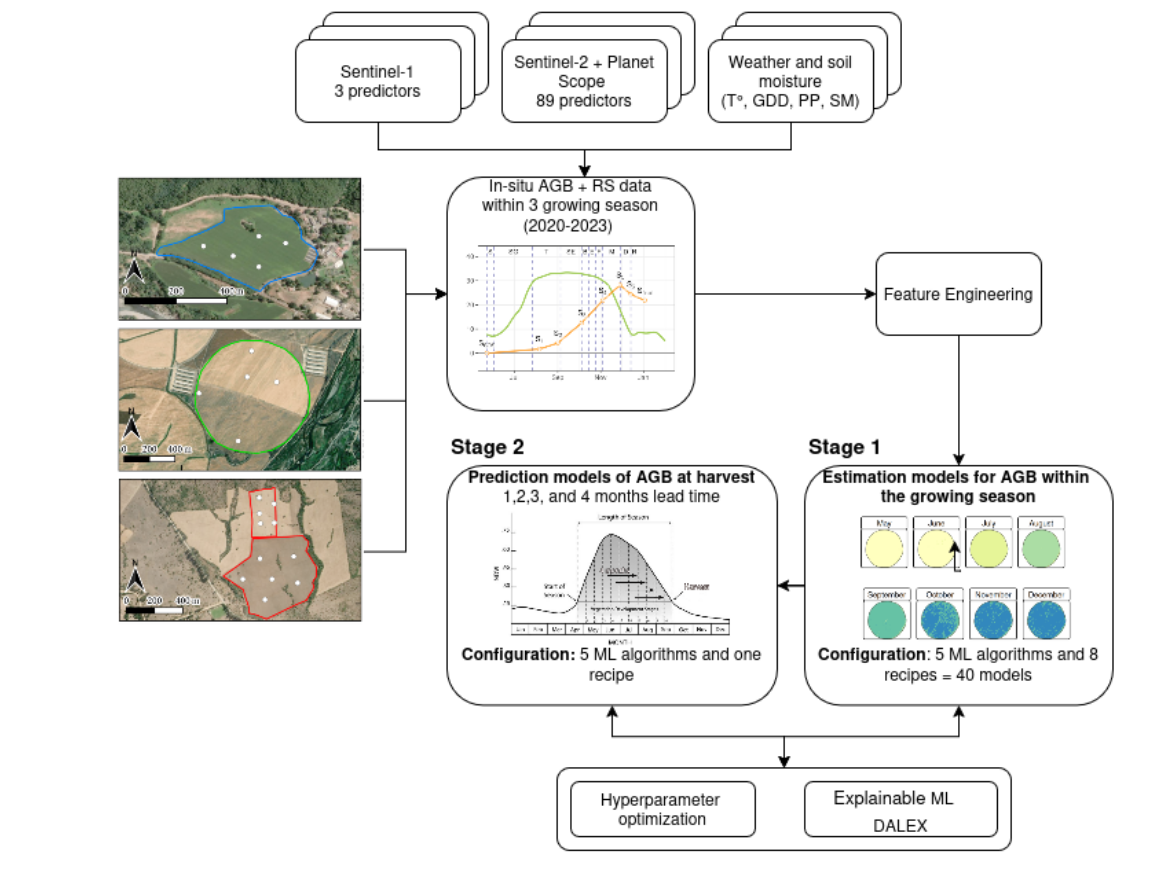
\includegraphics[width=1\linewidth,height=\textheight,keepaspectratio]{../output/figs/flowchart_diagram.png}

}

\caption{\label{fig-3}\textbf{Methodological scheme of the modeling
process by machine learning of the AGB estimation within the growing
season (stage 1) and the prediction at harvest at 1, 2, 3, and 4 month
lead times (stage 2).}}

\end{figure}%

Figure~\ref{fig-3} shows a general scheme for the modeling process. The
dataset for modeling is composed of the in situ AGB data and the remote
sensing predictors derived from S1, S2, and PlanetScope, as well as the
weather variables. All this data is generated as a time series for each
growing season in each site. Then a feature engineering process is
applied to the data before running the models. Thereafter, the dataset
is used in the first stage to run the ML models to estimate the
spatio-temporal variation of AGB within the growing season. After
achieving the initial results, we tested the ML prediction models of AGB
at harvest by using covariates from four lead times: 1, 2, 3, and 4
months. The ML models for estimation and prediction pass through a
hyperparameter optimization and an explainable ML process.

We tested five machine learning (ML) algorithms to estimate
spatio-temporal in-season and AGB (stage 1) and to predict AGB at
harvest (stage 2): extreme gradient boosting (XGBoost;
\citep{Chen2016}), random forest (RF; \citep{Ho1995}), regularized
generalized linear regression (GLMnet; \citep{Hastie2015}), single
layer, feed-forward neural networks (bagMLP; \citep{Breiman1996a}), and
K-nearest neighbors (KNN; \citep{Hechenbichler2004}). We also tested an
ensemble model which combines the predictions for the five models
\citep{Breiman1996c, Wolpert1992}. These models were selected based on
their robustness in regression tasks, capacity to handle
high-dimensional data, interpretability, and for being state-of-the-art.

\subsubsection{Defining dataset recipes for estimation and prediction
models}\label{defining-dataset-recipes-for-estimation-and-prediction-models}

The dataset used for the estimation modeling (stage 1) included
covariates derived from soil moisture data, weather variables, remote
sensing spectral information, and VIs. The response variable was AGB
(t/ha), obtained from field measurements. We split the predictor
variables into different subsets with the aim of evaluating
independently how weather, Sentinel-1, Sentinel-2, and PlanetScope
contribute to the estimation of AGB. We called each subset a recipe
(rec). Thus, \emph{rec1} used all the variables; \emph{rec2} uses only
Sentinel-1; \emph{rec3} uses Sentinel-1 and weather; \emph{rec4} uses
only weather variables; \emph{rec5} uses only Sentinel-2; \emph{rec6}
uses Sentinel-2 and weather; \emph{rec7} uses only PlanetScope; and
\emph{rec8} uses PlanetScope and weather.

\subsubsection{Feature engineering}\label{feature-engineering}

Before running the ML modeling for estimation and prediction, we applied
different preprocessing methods to the dataset. First, to fill missing
data, we imputed it using k-nearest neighbor \citep{Gower1971}. All of
the predictors were then normalized to have a standard deviation of one
and a mean of zero. Also, we applied a filter to eliminate highly
correlated variables (Pearson \textbar r\textbar{} ≥ 0.9), which removed
one of the 43 candidate predictors (S2\textsubscript{SWIR11}\_MCARI) for
\emph{rec1} in the stage 1 (estimation) dataset, leaving 42 predictors.
This correlation-based filter did not remove any variable from the stage
2 (prediction) dataset (Section 2.3.5), so all 43 candidate predictors
were retained for \emph{rec1} in stage 2. To document the residual
multicollinearity in the full predictor set, we additionally computed
variance inflation factors (VIF) on the 42 stage 1 predictors and
iteratively removed variables with VIF \textgreater{} 10, which reduced
the set to 22 variables. This VIF audit was performed for transparency
only and was not applied as a modeling step, since the regularized
(GLMnet) and tree-based (RF, XGBoost) algorithms used here are tolerant
of collinearity among spectral indices; the full audit is provided in
the project repository. While collinearity among spectral indices does
not bias point predictions from regularized or tree-based models, it
does affect permutation-based variable importance (Section 2.3.8):
permuting one of a set of mutually correlated predictors while holding
the others fixed generates combinations of values that are not jointly
observed in the training data, which can distort the resulting
importance and partial-dependence estimates. The importance results
presented below (Section 3.1.2) should therefore be interpreted as
indicating groups of mutually-informative, partly redundant predictors
rather than as precisely localized rankings of individual variables; the
VIF-reduced 22-variable set identified here provides a natural starting
point for a future reanalysis using conditional permutation importance
or VIF-reduced predictor sets (see Discussion, Study limitations).

\subsubsection{Estimation models for AGB within the growing
season}\label{estimation-models-for-agb-within-the-growing-season}

For the estimation model (stage 1), covariates from the same day as the
AGB measured in situ were employed. Thus, we generate a modeling dataset
by including the value of the covariates for each sample point. We used
a combination of 40 models, corresponding to the eight recipes
multiplied by the five ML algorithms. We then ran the models, tuned them
through hyperparameter optimization (see section 2.3.6), and used them
to estimate AGB spatially for each day and site during the growing
season. This process yields a daily spatiotemporal dataset of AGB for
each site.

\subsubsection{Prediction models for AGB at
harvest}\label{prediction-models-for-agb-at-harvest}

From the estimation modeling (stage 1), we obtained the daily
spatio-temporal AGB within the growing season. For prediction, we took
the AGB of the harvest date per site as the response variable; this
harvest-date AGB corresponds to the stage 1 model's spatial prediction
(Section 2.3.4) for each site-season, rather than an additional in-situ
destructive sample collected specifically at harvest. Consequently, the
stage 2 models are trained and evaluated against a model-derived
quantity rather than an independent ground-truth measurement: they test
whether remote-sensing and weather covariates available one to four
months before harvest are sufficient to reproduce the stage 1 model's
own spatial output at the harvest date, not whether they can forecast
actual, field-measured AGB at harvest. We therefore treat stage 2
throughout this study as an internal-consistency, proof-of-concept
analysis of the modeling pipeline rather than as an independent
validation of harvest-forecasting skill against ground truth;
establishing the latter would require a dedicated destructive-sampling
campaign at harvest, which was outside the scope of the present field
campaigns (see Discussion, Study limitations). As covariates, we
selected the remote sensing covariates (S1, S2, and PS variables in
Table~Table~\ref{tbl-3}) and weather data, which lagged from one to four
months before harvesting as lead time. To generate the dataset for
prediction modeling, we took 100 random samples per site for the
responses and covariates. These 100 samples per site-season capture
within-field spatial variation in the modeled harvest-date AGB and the
corresponding predictor surfaces around a single harvest date; because
the leave-one-site-out cross-validation scheme (Section 2.3.6) holds out
all samples belonging to a given site-season as one block, this
within-site resampling does not leak information across folds. However,
because these 100 points are drawn from a smoothed,
spatially-autocorrelated stage 1 prediction surface rather than from
independent biological replicates, they are not 100 independent
observations: the resulting dataset (400 points across the four
site-seasons) carries substantial redundancy, so its nominal size should
be regarded as an upper bound on the effective sample size, and the
stage 2 performance metrics reported below (Section 3.2) may understate
the uncertainty that would be obtained with independent harvest-date
samples. In the modeling process, we used hyperparameter optimization to
enhance the performance of our models and then applied them to predict
aboveground biomass (AGB) at harvest for each lead time.

\subsubsection{Hyperparameter optimization and
evaluation}\label{hyperparameter-optimization-and-evaluation}

To tune each parameter per algorithm for the estimation and prediction
modeling, we used hyperparameter optimization, defining ten random
candidates per parameter combination (Table~Table~\ref{tbl-4}). For the
estimation models (stage 1), performance was evaluated using a
leave-one-site-out cross-validation (LOSO-CV) scheme, in which the data
were partitioned into four folds, each corresponding to one of the four
site-seasons (Hidango 2021--2022, Hidango 2022--2023, La Cancha
2022--2023, and Villa Baviera 2020--2021). For each recipe-algorithm
combination, the ten hyperparameter candidates were fitted on the three
remaining site-seasons and evaluated on the held-out site-season; the
configuration with the highest mean R² across the four folds was
selected, and its corresponding mean R², RMSE, and MAE across folds were
retained as the final performance estimate. This LOSO scheme directly
evaluates the spatial transferability of each model to a field/season
not used for training, which is the most policy-relevant generalization
scenario for operational AGB monitoring. We note that, because the
held-out site-season is used both to select the best-performing
hyperparameter configuration and to report that configuration's
performance, this procedure does not provide a fully nested estimate of
generalization error: the reported R², RMSE, and MAE for each
recipe-algorithm combination may be optimistically biased relative to a
strictly nested LOSO-CV, in which hyperparameter selection would be
confined to the three training site-seasons only (e.g., via an inner
cross-validation loop). We retain this non-nested scheme because, with
only four site-seasons, an inner-loop split would leave too few
independent units per fold; we therefore interpret the reported metrics
primarily as a basis for relative comparison among recipes and
algorithms---all of which are subject to the same selection procedure
and thus the same potential bias---rather than as unbiased absolute
estimates of out-of-sample performance. The complementary
sensor-ablation analysis (Table Table~\ref{tbl-6}), which uses fixed
hyperparameters and is therefore not subject to this selection-based
optimism, corroborates the recipe-level ranking (Section 3.1.1),
providing some reassurance that the qualitative conclusions are not
solely an artifact of this leakage; we discuss this limitation further,
including the need for nested cross-validation in future work, in the
Discussion (Study limitations). For the prediction models (stage 2), the
same LOSO-CV scheme was applied to the
100-random-samples-per-site-per-lead-time dataset, using recipe
\emph{rec1} (all predictors) combined with five algorithms (RF, XGBoost,
GLMnet, bagMLP, and KNN). For each lead time and algorithm, the ten
hyperparameter candidates were evaluated across the four LOSO folds and
the configuration with the highest mean R² across folds was retained,
with its mean R², RMSE, and MAE across folds reported as the final
performance estimate; selected models were then refit on the complete
dataset using the chosen hyperparameters. We used the mean absolute
error (MAE), root mean square error (RMSE), and r-squared (R²) metrics
(see Supplementary Material Eqs. S1, S2 \& S3).

\subsubsection{Stacked ensemble model}\label{stacked-ensemble-model}

In addition to the 40 individual recipe-algorithm combinations evaluated
via LOSO-CV, we built a stacked ensemble model following
\citep{Breiman1996c} and \citep{Wolpert1992}. Using the \{stacks\}
package \citep{Couch2022}, the tuned candidates from the stage 1
workflow set were supplied as ensemble members; a LASSO meta-learner
(penalized linear regression) was fitted on their out-of-fold
predictions to estimate blending weights, retaining only members with a
non-zero coefficient. The selected members were then refit on the
complete dataset (all four site-seasons, recipe \emph{rec1}, all
predictors) to produce the final ensemble model, which was used as the
basis for the explainable ML analysis described below.

\begin{longtable}[]{@{}
  >{\raggedright\arraybackslash}p{(\linewidth - 4\tabcolsep) * \real{0.3191}}
  >{\raggedright\arraybackslash}p{(\linewidth - 4\tabcolsep) * \real{0.3617}}
  >{\raggedright\arraybackslash}p{(\linewidth - 4\tabcolsep) * \real{0.3191}}@{}}
\caption{Parameters per machine learning algorithm. RF: random forest.
XGBoost: extreme gradient boosting. GLMnet: regularized generalized
linear regression. BAGmlp: single layer, feed-forward neural networks.
KNN: k-nearest neighbour. *This parameter was not
tuned.}\label{tbl-4}\tabularnewline
\toprule\noalign{}
\begin{minipage}[b]{\linewidth}\raggedright
\textbf{Parameter}
\end{minipage} & \begin{minipage}[b]{\linewidth}\raggedright
\textbf{Description}
\end{minipage} & \begin{minipage}[b]{\linewidth}\raggedright
\textbf{Algorithm}
\end{minipage} \\
\midrule\noalign{}
\endfirsthead
\toprule\noalign{}
\begin{minipage}[b]{\linewidth}\raggedright
\textbf{Parameter}
\end{minipage} & \begin{minipage}[b]{\linewidth}\raggedright
\textbf{Description}
\end{minipage} & \begin{minipage}[b]{\linewidth}\raggedright
\textbf{Algorithm}
\end{minipage} \\
\midrule\noalign{}
\endhead
\bottomrule\noalign{}
\endlastfoot
trees* & An integer for the number of trees contained in the ensemble.
Fixed to 1000 trees. & XGBoost, RF \\
tree\_depth & An integer for the maximum depth of the tree. & XGBoost,
RF \\
min\_n & An integer for the minimum number of data points in a node that
is required for the node to be split further. & XGBoost, RF \\
loss\_reduction & A number for the reduction in the loss function
required to split further. & XGBoost \\
sample\_size & A number for the number (or proportion) of data that is
exposed to the fitting routine. & XGBoost \\
learn\_rate & A number for the rate at which the boosting algorithm
adapts from iteration-to-iteration. & XGBoost \\
mtry & An integer for the number of predictors that are randomly sampled
at each split when creating tree models. & XGBoost, RF \\
penalty & A non-negative number representing the total amount of
regularization. & GLMnet, bagMLP \\
mixture & A number between zero and one (inclusive) denoting the
proportion of L1 regularization (i.e.~lasso) in the model. & GLMnet \\
hidden units & An integer for the number of units in the hidden model. &
bagMLP \\
epochs & An integer for the number of training iterations. & BagMLP \\
neighbors & The number of neighbors to consider (often called k) &
KNN \\
weight\_func & A single character for the type of kernel function used
to weight distances between samples. & KNN \\
dist\_power & A single number for the parameter used in calculating
Minkowski distance. & KNN \\
\end{longtable}

\subsubsection{Explainable Machine Learning with
DALEX}\label{explainable-machine-learning-with-dalex}

To assess the contribution of each covariate to the model's performance,
we performed a variable importance analysis. Further, to evaluate how
the most important variables impact the model's predictions, we used
partial dependence plots. For this, we used the DALEX (moDel Agnostic
Language for Exploration and eXplanation). DALEX provides a
model-agnostic framework for interpreting machine learning models by
quantifying the impact of individual variables on model predictions. We
computed permutation-based variable importance, which evaluates the
increase in prediction error after permuting the values of a given
variable while keeping all other variables fixed. This approach captures
both main effects and interactions and is applicable across diverse
model types. For estimation, we analyzed the ensemble model that used
all the predictors (recipe \emph{rec1}), and for prediction, we used the
best model for each lead time. For each variable, we calculated the
increase in root mean squared error (ΔRMSE) caused by the permutation.
Higher ΔRMSE values indicate greater importance of the corresponding
variable to model performance. The analysis was repeated over 50 random
permutations to ensure stability of the importance rankings. The top
predictors were identified by ranking variables based on the mean ΔRMSE.
In addition, we calculated a ``scaled dropout loss'' metric to compare
variable influence across lead times in the prediction models.

\subsection{Software}\label{software}

We utilized the R programming language \citep{RCoreTeam2025} for
processing satellite data, as well as for data analysis, ML modeling,
and visualization. To access satellite data, we employed the
\{earthdatalogin\} package \citep{Boettiger2023}. For smoothing the time
series of vegetation indices, we applied the \{imputeTS\} package
\citep{Moritz2017}. We used the \{terra\} package \citep{Hijmans2023}
and the \{sf\} package \citep{Pebesma2018} for processing raster and
vectorial data. For data science tasks and visualization, we utilized
the \{tidyverse\} suite \citep{Wickham2019}. For machine learning
modeling, we work with the \{tidymodels\} framework \citep{Kuhn2020}.
For the variable importance we used \{DALEX\} \citep{Biecek2018}. The
\{tmap\} package \citep{Tennekes2018} was employed for mapping purposes.

\section{Results}\label{results}

\subsection{Estimation model for AGB within the growing
season}\label{estimation-model-for-agb-within-the-growing-season}

\subsubsection{Selecting the best
models}\label{selecting-the-best-models}

For AGB estimation, we tested 40 models generated by a combination of
five machine learning algorithms and eight recipes, each evaluated using
leave-one-site-out cross-validation (LOSO-CV) across the four
site-seasons. Across the 40 models, R² ranged from 0.44 to 0.78, MAE
from 5.2 to 9.0 t/ha, and RMSE from 6.7 to 10.2 t/ha
(Figure~\ref{fig-4}). RF and XGBoost were generally the best-performing
algorithms, while GLMnet was the weakest overall. The recipe
\emph{rec7}, which uses only PlanetScope (PS) predictors, ranked first
with RF (R²=0.78±0.08, RMSE=7.87±2.08 t/ha, MAE=5.90±2.32 t/ha; mean±SD
across the four LOSO folds) and second with XGBoost (R²=0.77, RMSE=7.55
t/ha, MAE=5.75 t/ha); \emph{rec8} (PS+weather) ranked third and fourth
with XGBoost and RF, respectively. By contrast, \emph{rec2} (S1 only)
consistently ranked among the worst recipes regardless of algorithm
(ranks 36-40 of 40, R²=0.44-0.53), with its GLMnet configuration ranking
last overall---indicating that Sentinel-1 backscatter alone carries
little transferable information about AGB across sites and seasons. The
recipe that incorporates all covariates (\emph{rec1}) did not outperform
the PlanetScope-only recipes; its best configuration (bagMLP) ranked
sixth overall (R²=0.75, RMSE=6.96 t/ha, MAE=5.34 t/ha). This pattern is
corroborated by an independent sensor-ablation analysis (Table
Table~\ref{tbl-6}), in which adding Sentinel-1 to a Sentinel-2+weather
model changed RMSE by only +0.5\% (i.e., a marginal degradation),
whereas adding PlanetScope to a Sentinel-1+Sentinel-2+weather model
improved RMSE by 5.7\%.

\begin{figure}

\centering{

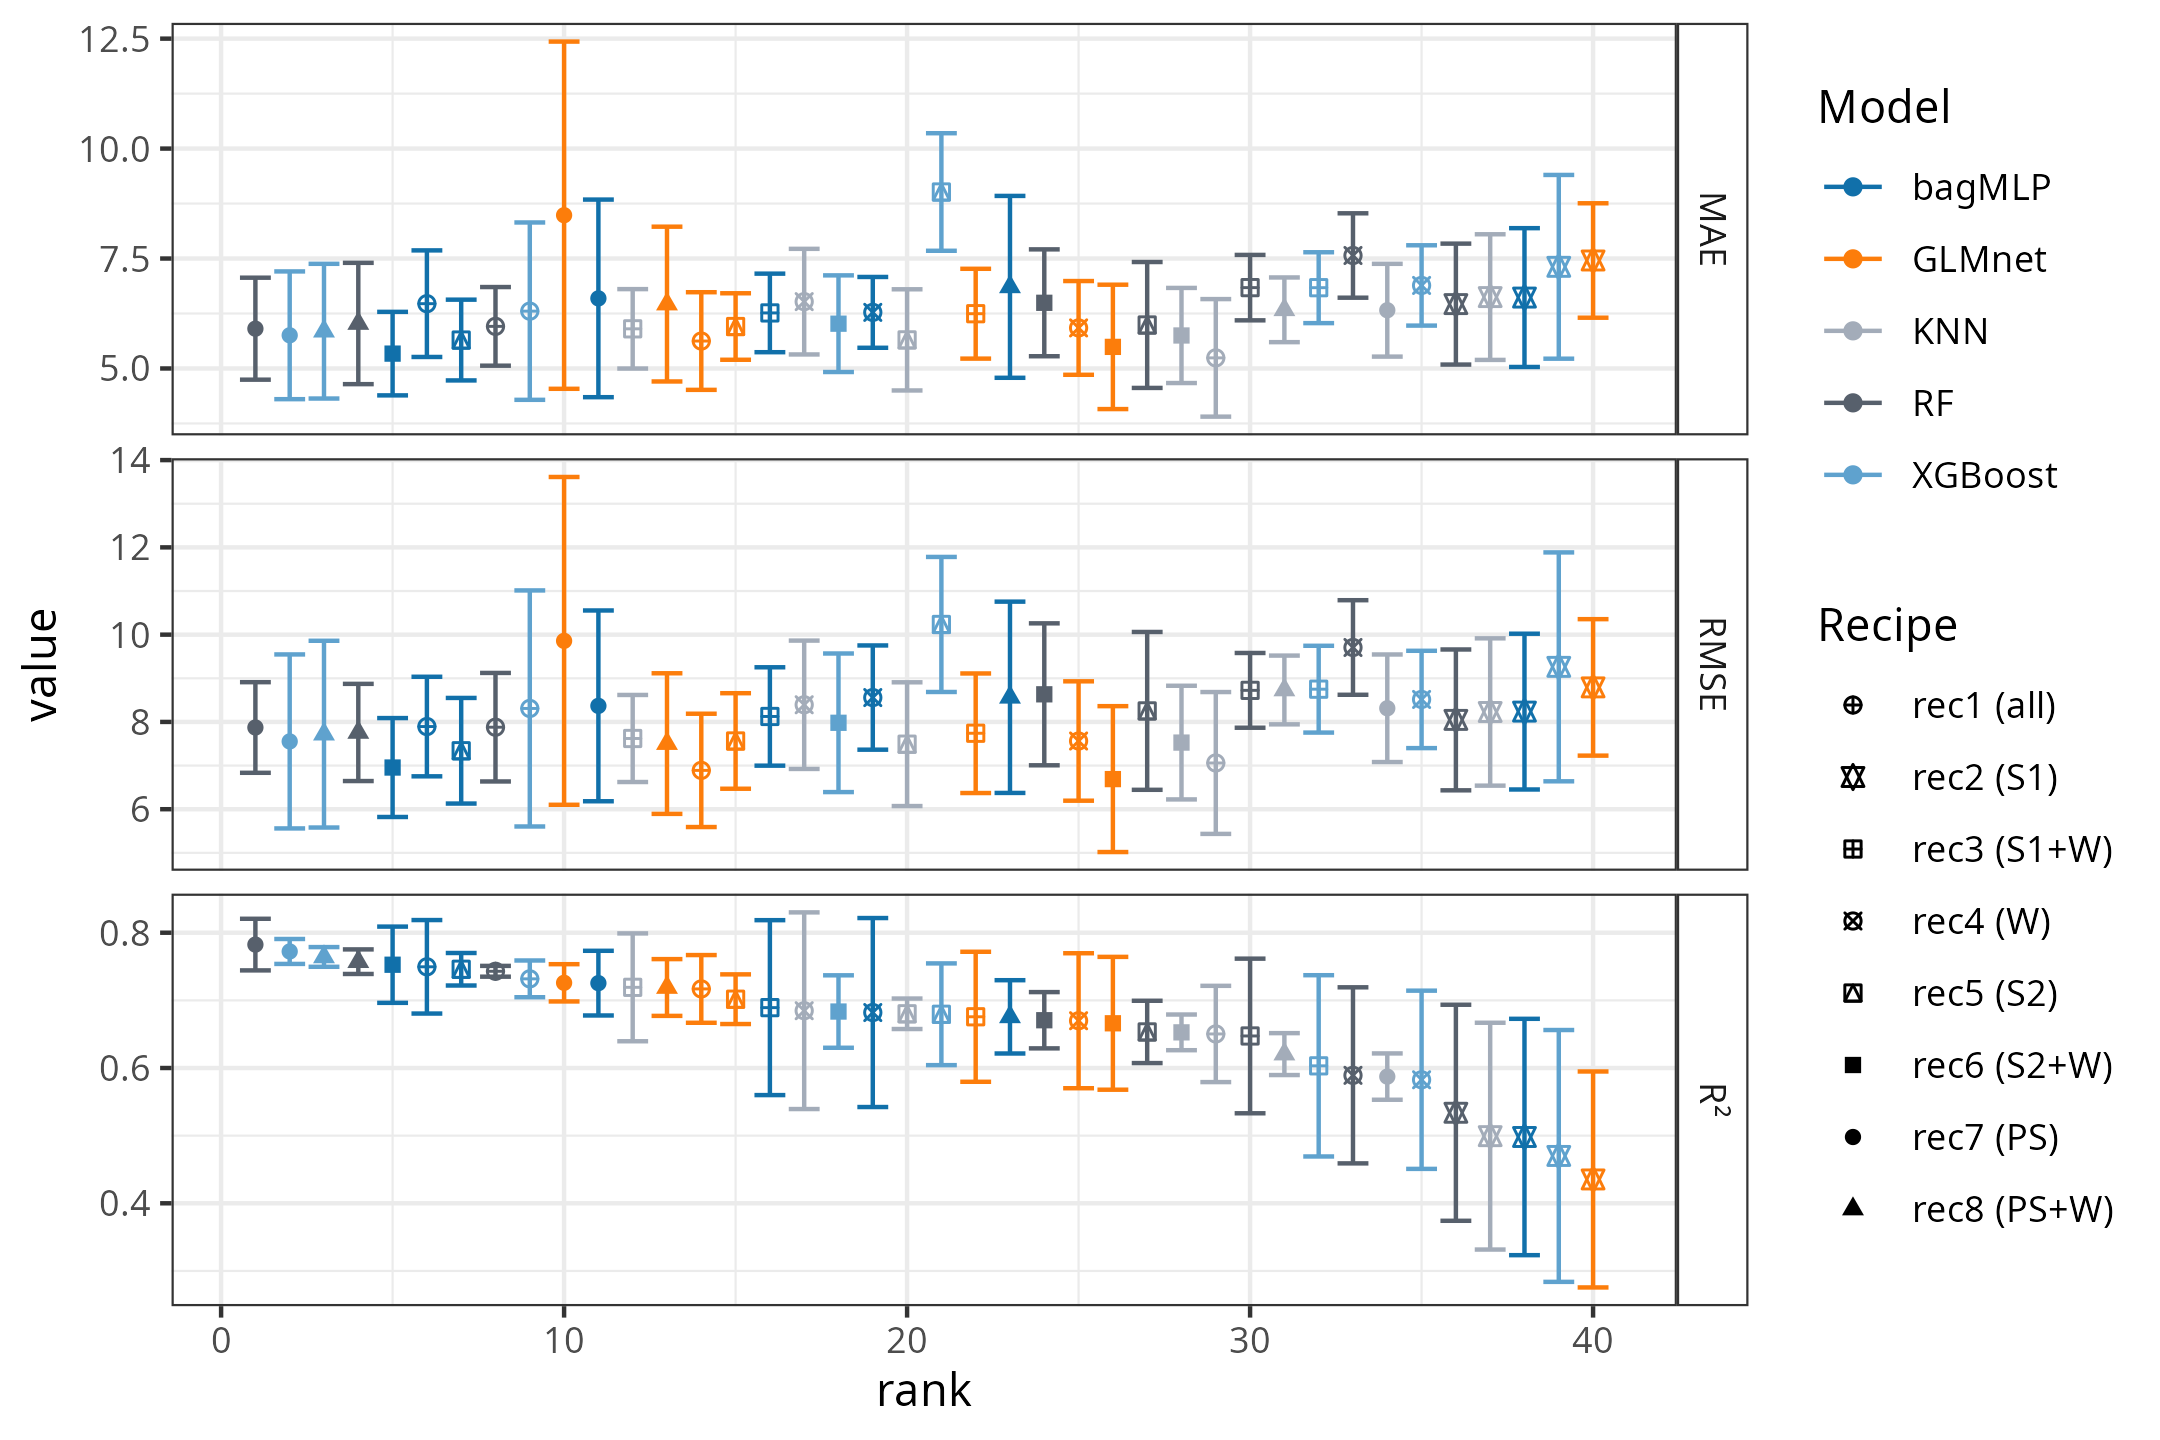
\includegraphics[width=1\linewidth,height=\textheight,keepaspectratio]{../output/figs/ranking_estimacion_modelos_rec.png}

}

\caption{\label{fig-4}\textbf{Performance metrics (R², MAE, and RMSE)
for the forty models (five ML algorithms and eight recipes), ranked from
best to worst under leave-one-site-out cross-validation.} RF: random
forest, KNN: k-nearest neighbor, XGBoost: extreme gradient boosting,
GLMnet: generalized linear models with regularization, bagMLP:
feed-forward neural networks. rec1: all predictors, rec2: Sentinel-1
(S1), rec3: S1+weather (W), rec4: weather only, rec5: Sentinel-2 (S2),
rec6: S2+W, rec7: PlanetScope (PS), rec8: PS+W.}

\end{figure}%

Figure~\ref{fig-5} compares observed and out-of-fold predicted AGB for
the top-ranked configuration (\emph{rec7}\_RF, PlanetScope only), its
runner-up (\emph{rec7}\_XGBoost), and a representative all-predictors
configuration (\emph{rec1}\_RF, rank 8 overall, R²=0.74, RMSE=7.88 t/ha)
for context. The PlanetScope-only models track the 1:1 line closely
across the full biomass range, including the high-biomass observations
(\textgreater25 t/ha) where the all-predictors model shows a tendency to
underestimate.

\begin{figure}

\centering{

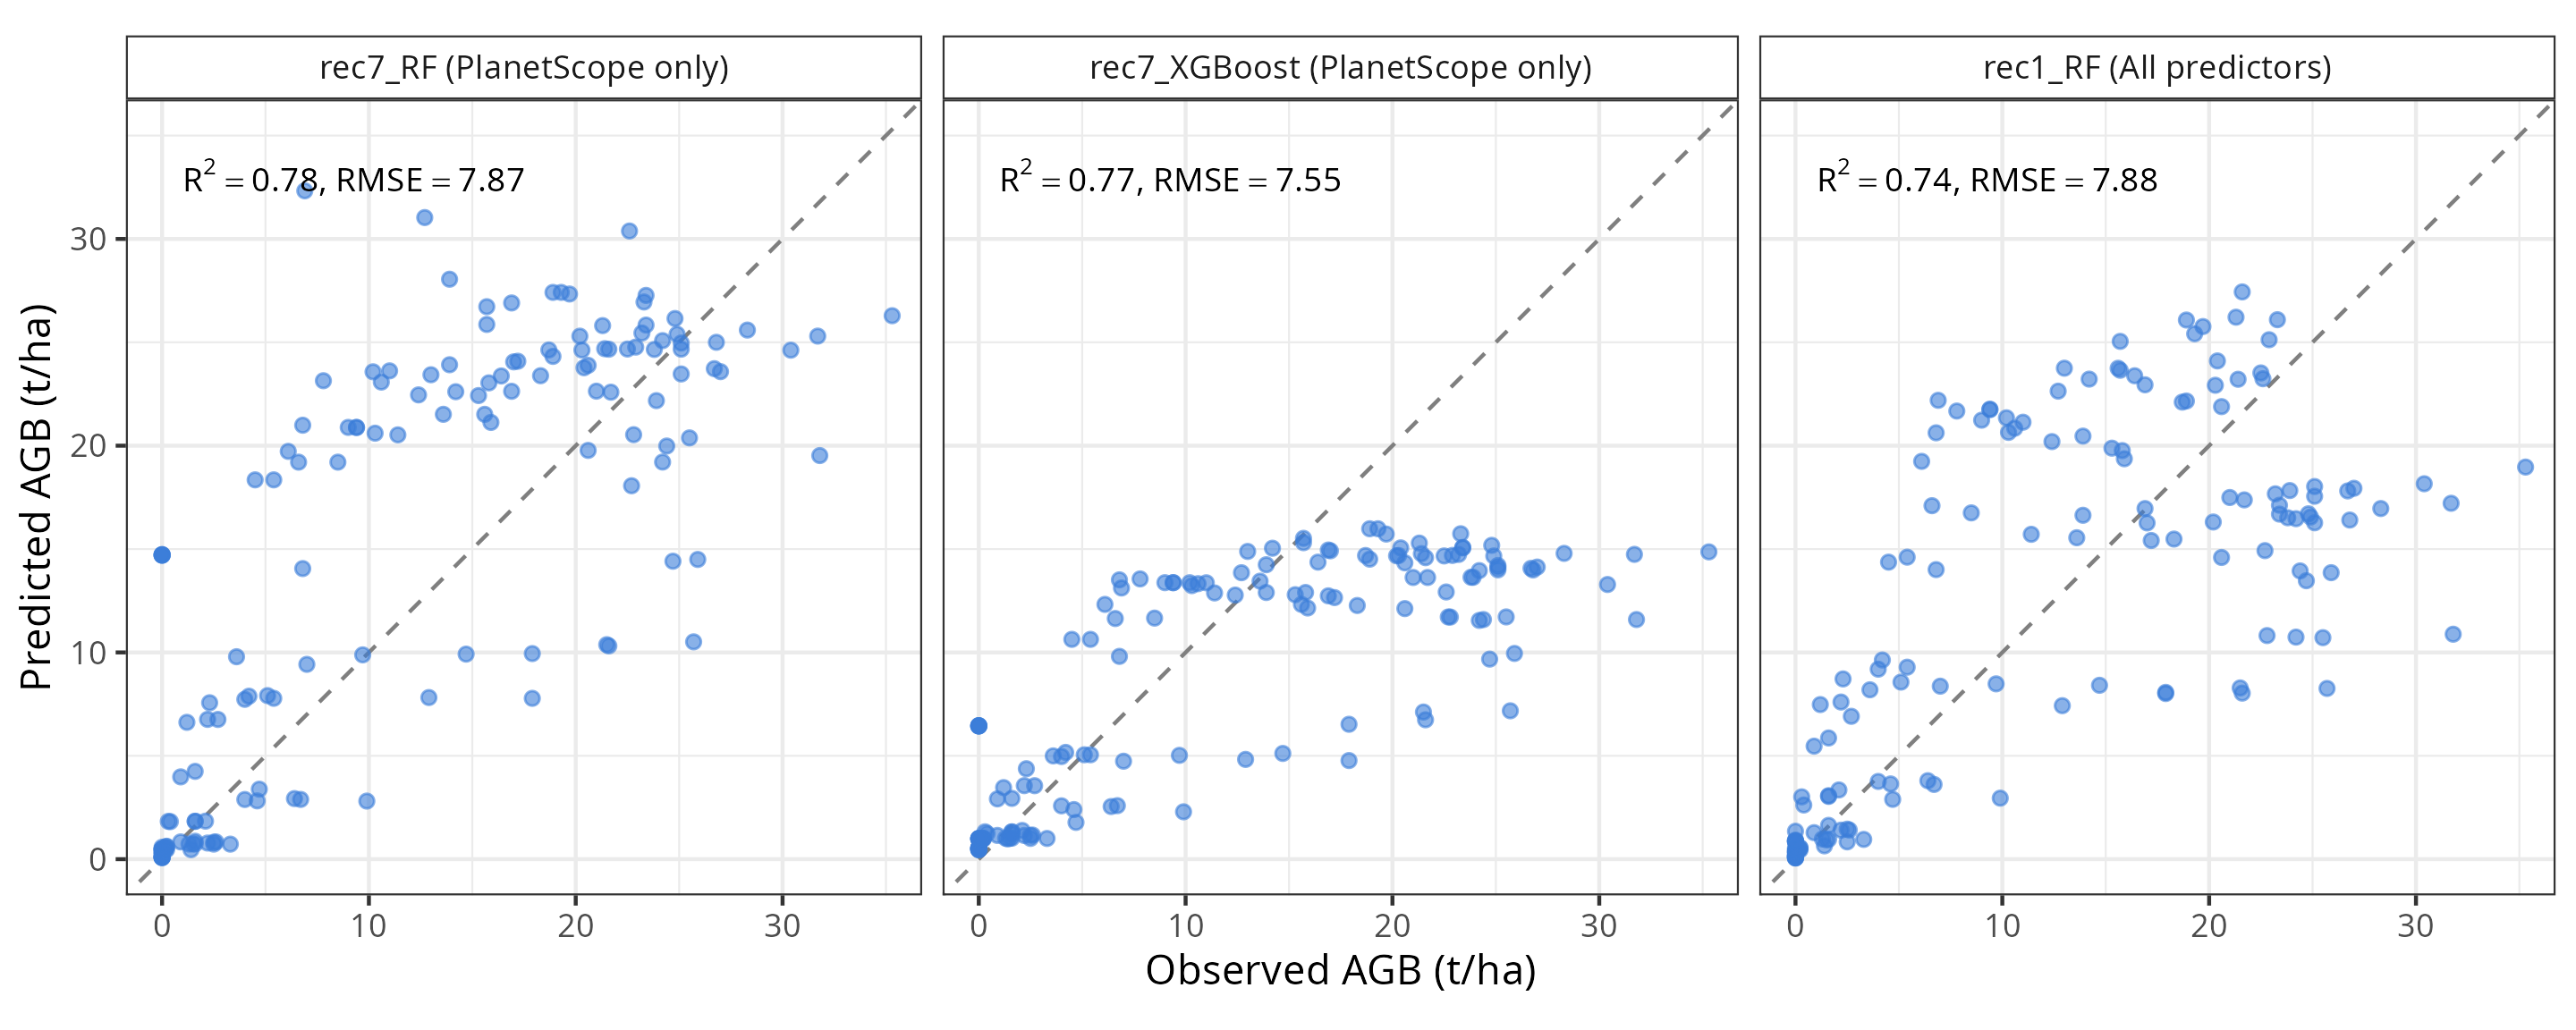
\includegraphics[width=1\linewidth,height=\textheight,keepaspectratio]{../output/figs/estimation_vs_observed_AGB_LOSO.png}

}

\caption{\label{fig-5}\textbf{Comparison of observed and out-of-fold
predicted aboveground biomass (LOSO-CV) for the top-ranked models.} R²
and RMSE correspond to the official ranking (mean across the four LOSO
folds, best hyperparameter configuration).}

\end{figure}%

As an independent check on the recipe ranking above, we ran a
complementary sensor-ablation analysis with fixed-hyperparameter XGBoost
models---fixed hyperparameters were used here, rather than the
per-recipe tuned configurations underlying Figure~\ref{fig-4}, to
isolate the marginal effect of each sensor group from
hyperparameter-tuning variance---under the same LOSO-CV scheme,
sequentially adding sensor groups to a weather-only baseline (Table
Table~\ref{tbl-6}). Adding Sentinel-2 to the weather-only model reduced
RMSE by 23.4\%, confirming the strong contribution of optical vegetation
indices. Adding Sentinel-1 to the Sentinel-2+weather model produced a
negligible change in RMSE (+0.5\%, i.e., a slight degradation), while
subsequently adding PlanetScope reduced RMSE by a further 5.7\%. This
independent analysis is consistent with the recipe ranking in
Figure~\ref{fig-4}: optical sensors (Sentinel-2 and PlanetScope) drive
most of the predictive performance, whereas Sentinel-1 SAR backscatter
contributes little once optical and weather information are available.
As Table Table~\ref{tbl-6} shows, the across-fold SD for each
configuration (2.6-3.4 t/ha) is substantial relative to these mean
differences, underscoring that with only four LOSO folds these ablation
effects---particularly the near-zero Sentinel-1 contribution---should be
interpreted as indicative rather than statistically definitive.

\begin{longtable}[]{@{}
  >{\raggedright\arraybackslash}p{(\linewidth - 6\tabcolsep) * \real{0.2500}}
  >{\raggedright\arraybackslash}p{(\linewidth - 6\tabcolsep) * \real{0.2500}}
  >{\raggedright\arraybackslash}p{(\linewidth - 6\tabcolsep) * \real{0.2500}}
  >{\raggedright\arraybackslash}p{(\linewidth - 6\tabcolsep) * \real{0.2500}}@{}}
\caption{Sensor-ablation analysis. Each row reports the change in mean
LOSO-CV RMSE (fixed-hyperparameter XGBoost) when a sensor group is added
sequentially to the previous model. RMSE values are mean ± SD across the
four LOSO folds.}\label{tbl-6}\tabularnewline
\toprule\noalign{}
\begin{minipage}[b]{\linewidth}\raggedright
\textbf{Sensor added}
\end{minipage} & \begin{minipage}[b]{\linewidth}\raggedright
\textbf{RMSE before (t/ha)}
\end{minipage} & \begin{minipage}[b]{\linewidth}\raggedright
\textbf{RMSE after (t/ha)}
\end{minipage} & \begin{minipage}[b]{\linewidth}\raggedright
\textbf{RMSE change (\%)}
\end{minipage} \\
\midrule\noalign{}
\endfirsthead
\toprule\noalign{}
\begin{minipage}[b]{\linewidth}\raggedright
\textbf{Sensor added}
\end{minipage} & \begin{minipage}[b]{\linewidth}\raggedright
\textbf{RMSE before (t/ha)}
\end{minipage} & \begin{minipage}[b]{\linewidth}\raggedright
\textbf{RMSE after (t/ha)}
\end{minipage} & \begin{minipage}[b]{\linewidth}\raggedright
\textbf{RMSE change (\%)}
\end{minipage} \\
\midrule\noalign{}
\endhead
\bottomrule\noalign{}
\endlastfoot
Sentinel-2 (vs.~weather only) & 9.96 ± 2.72 & 7.63 ± 3.43 & -23.4 \\
Sentinel-1 (vs.~Sentinel-2 + weather) & 7.63 ± 3.43 & 7.68 ± 3.00 &
+0.5 \\
PlanetScope (vs.~Sentinel-1 + Sentinel-2 + weather) & 7.68 ± 3.00 & 7.24
± 2.58 & -5.7 \\
\end{longtable}

\subsubsection{Explainable Machine Learning with
DALEX}\label{explainable-machine-learning-with-dalex-1}

\begin{figure}

\centering{

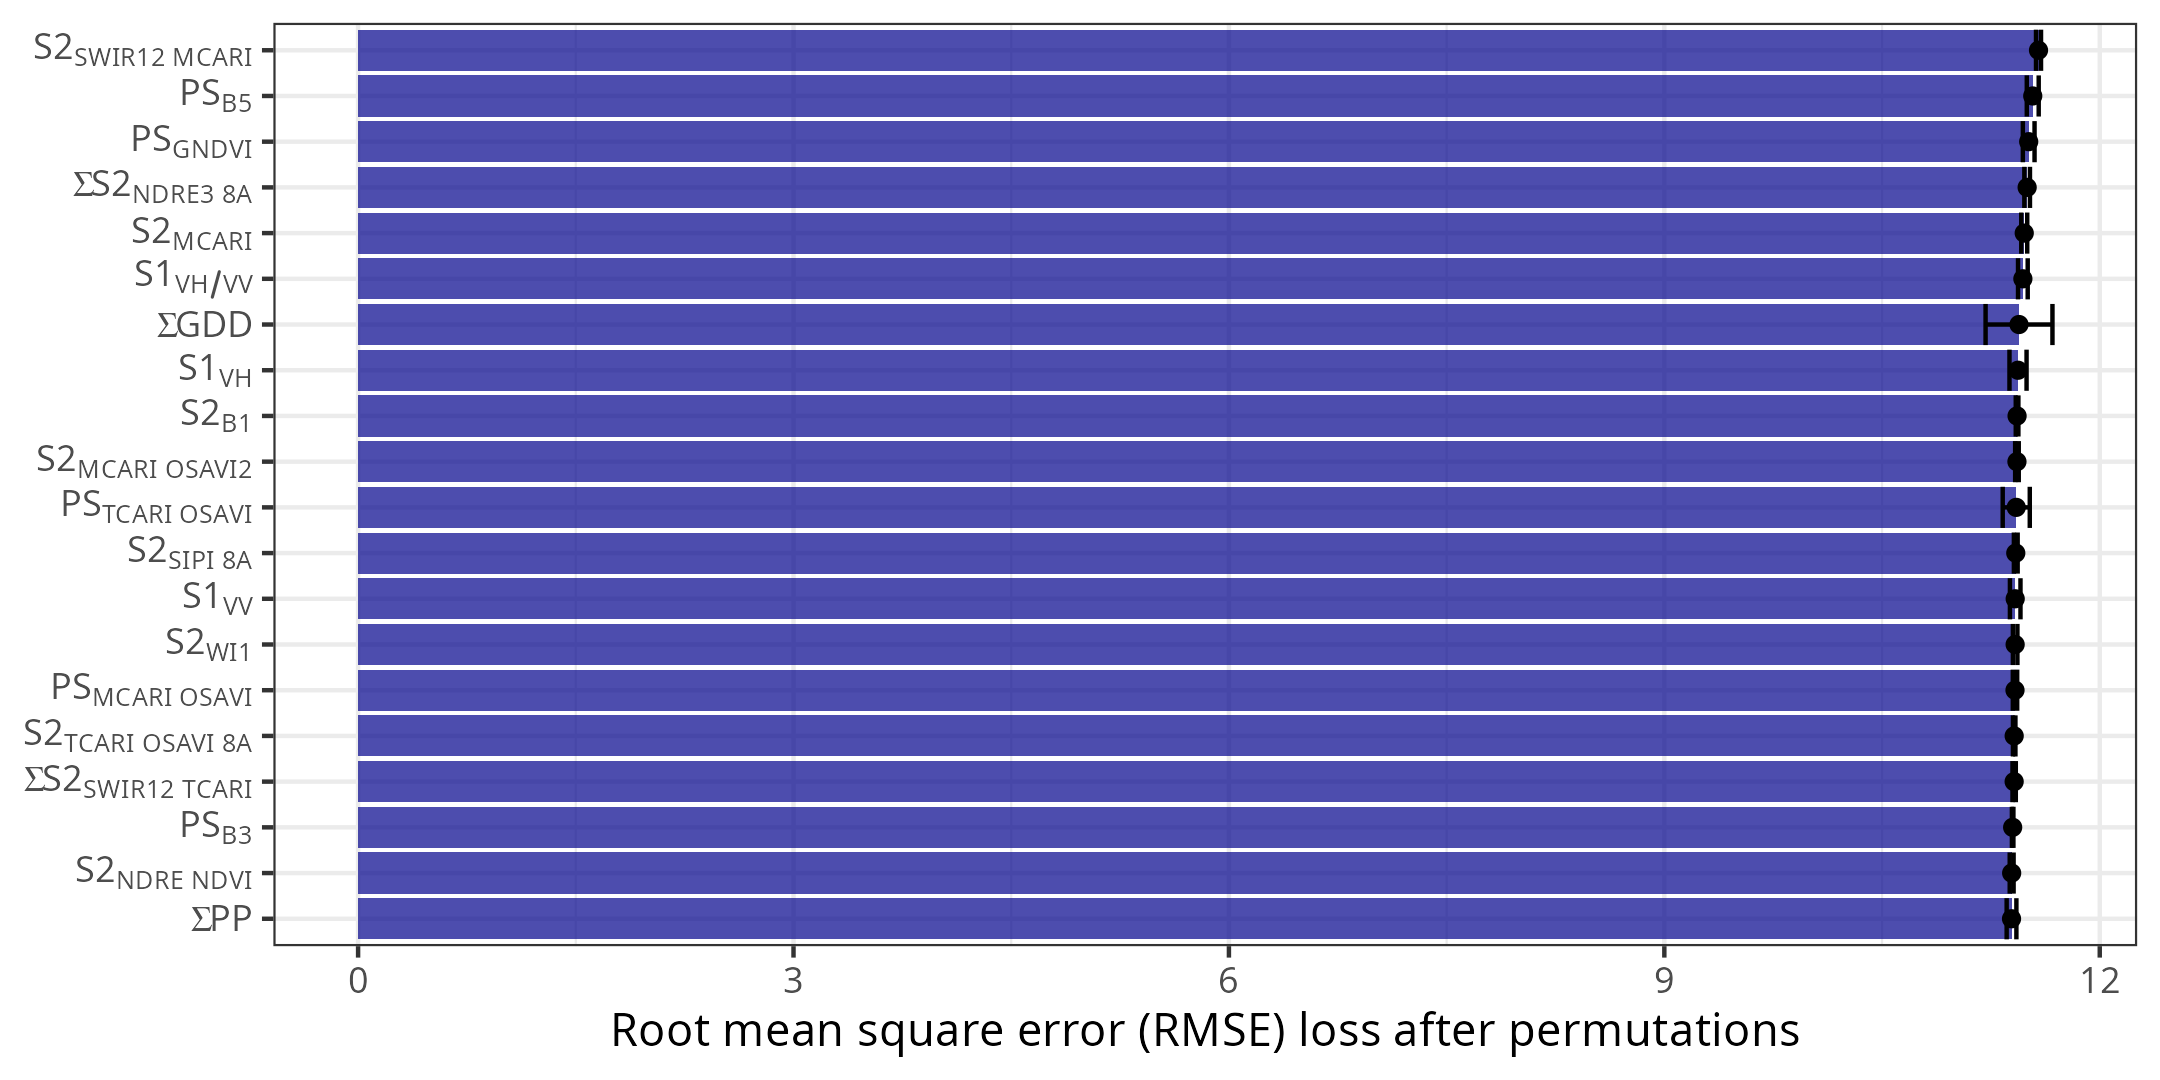
\includegraphics[width=1\linewidth,height=\textheight,keepaspectratio]{../output/figs/variables_importance_estimacion_modelo_ensamblado_LOSO.png}

}

\caption{\label{fig-6}\textbf{Optical (Sentinel-2, PlanetScope), SAR
(Sentinel-1), and accumulated thermal-time variables show comparable
impact on the LOSO-tuned ensemble model performance.} The twenty most
important variables, ranked by the increase in RMSE (dropout loss) after
permutation in the stacked ensemble model (recipe \emph{rec1}, all
predictors). Error bars show ±1 standard deviation across 50
permutations. The ∑ symbol indicates cumulative indices computed from
the start of the growing season.}

\end{figure}%

For the LOSO-tuned ensemble (recipe \emph{rec1}, all predictors),
permutation-based variable importance shows a relatively flat ranking
across the leading predictors (Figure~\ref{fig-6}): the Sentinel-2
SWIR-related chlorophyll index S2\textsubscript{SWIR12\_MCARI} ranks
highest, closely followed by two PlanetScope bands/indices
(PS\textsubscript{B5}, PS\textsubscript{GNDVI}), a cumulative Sentinel-2
red-edge index (∑S2\textsubscript{NDRE3\_8A}), S2\textsubscript{MCARI},
the Sentinel-1 backscatter ratio S1\textsubscript{VH/VV}, ∑GDD,
S1\textsubscript{VH}, S2\textsubscript{B1}, and
S2\textsubscript{MCARI/OSAVI2}---all within a narrow range of
dropout-loss values (11.4-11.6 RMSE units). Unlike the recipe-level
ranking in Figure~\ref{fig-4}, where PlanetScope-based recipes clearly
outperform the others, the ensemble-level importance indicates that
optical (S2, PS), SAR (S1), and accumulated thermal-time predictors all
contribute comparably once combined in a single model, consistent with
the residual collinearity documented by the VIF audit (Section 2.3.3).

\begin{figure}

\centering{

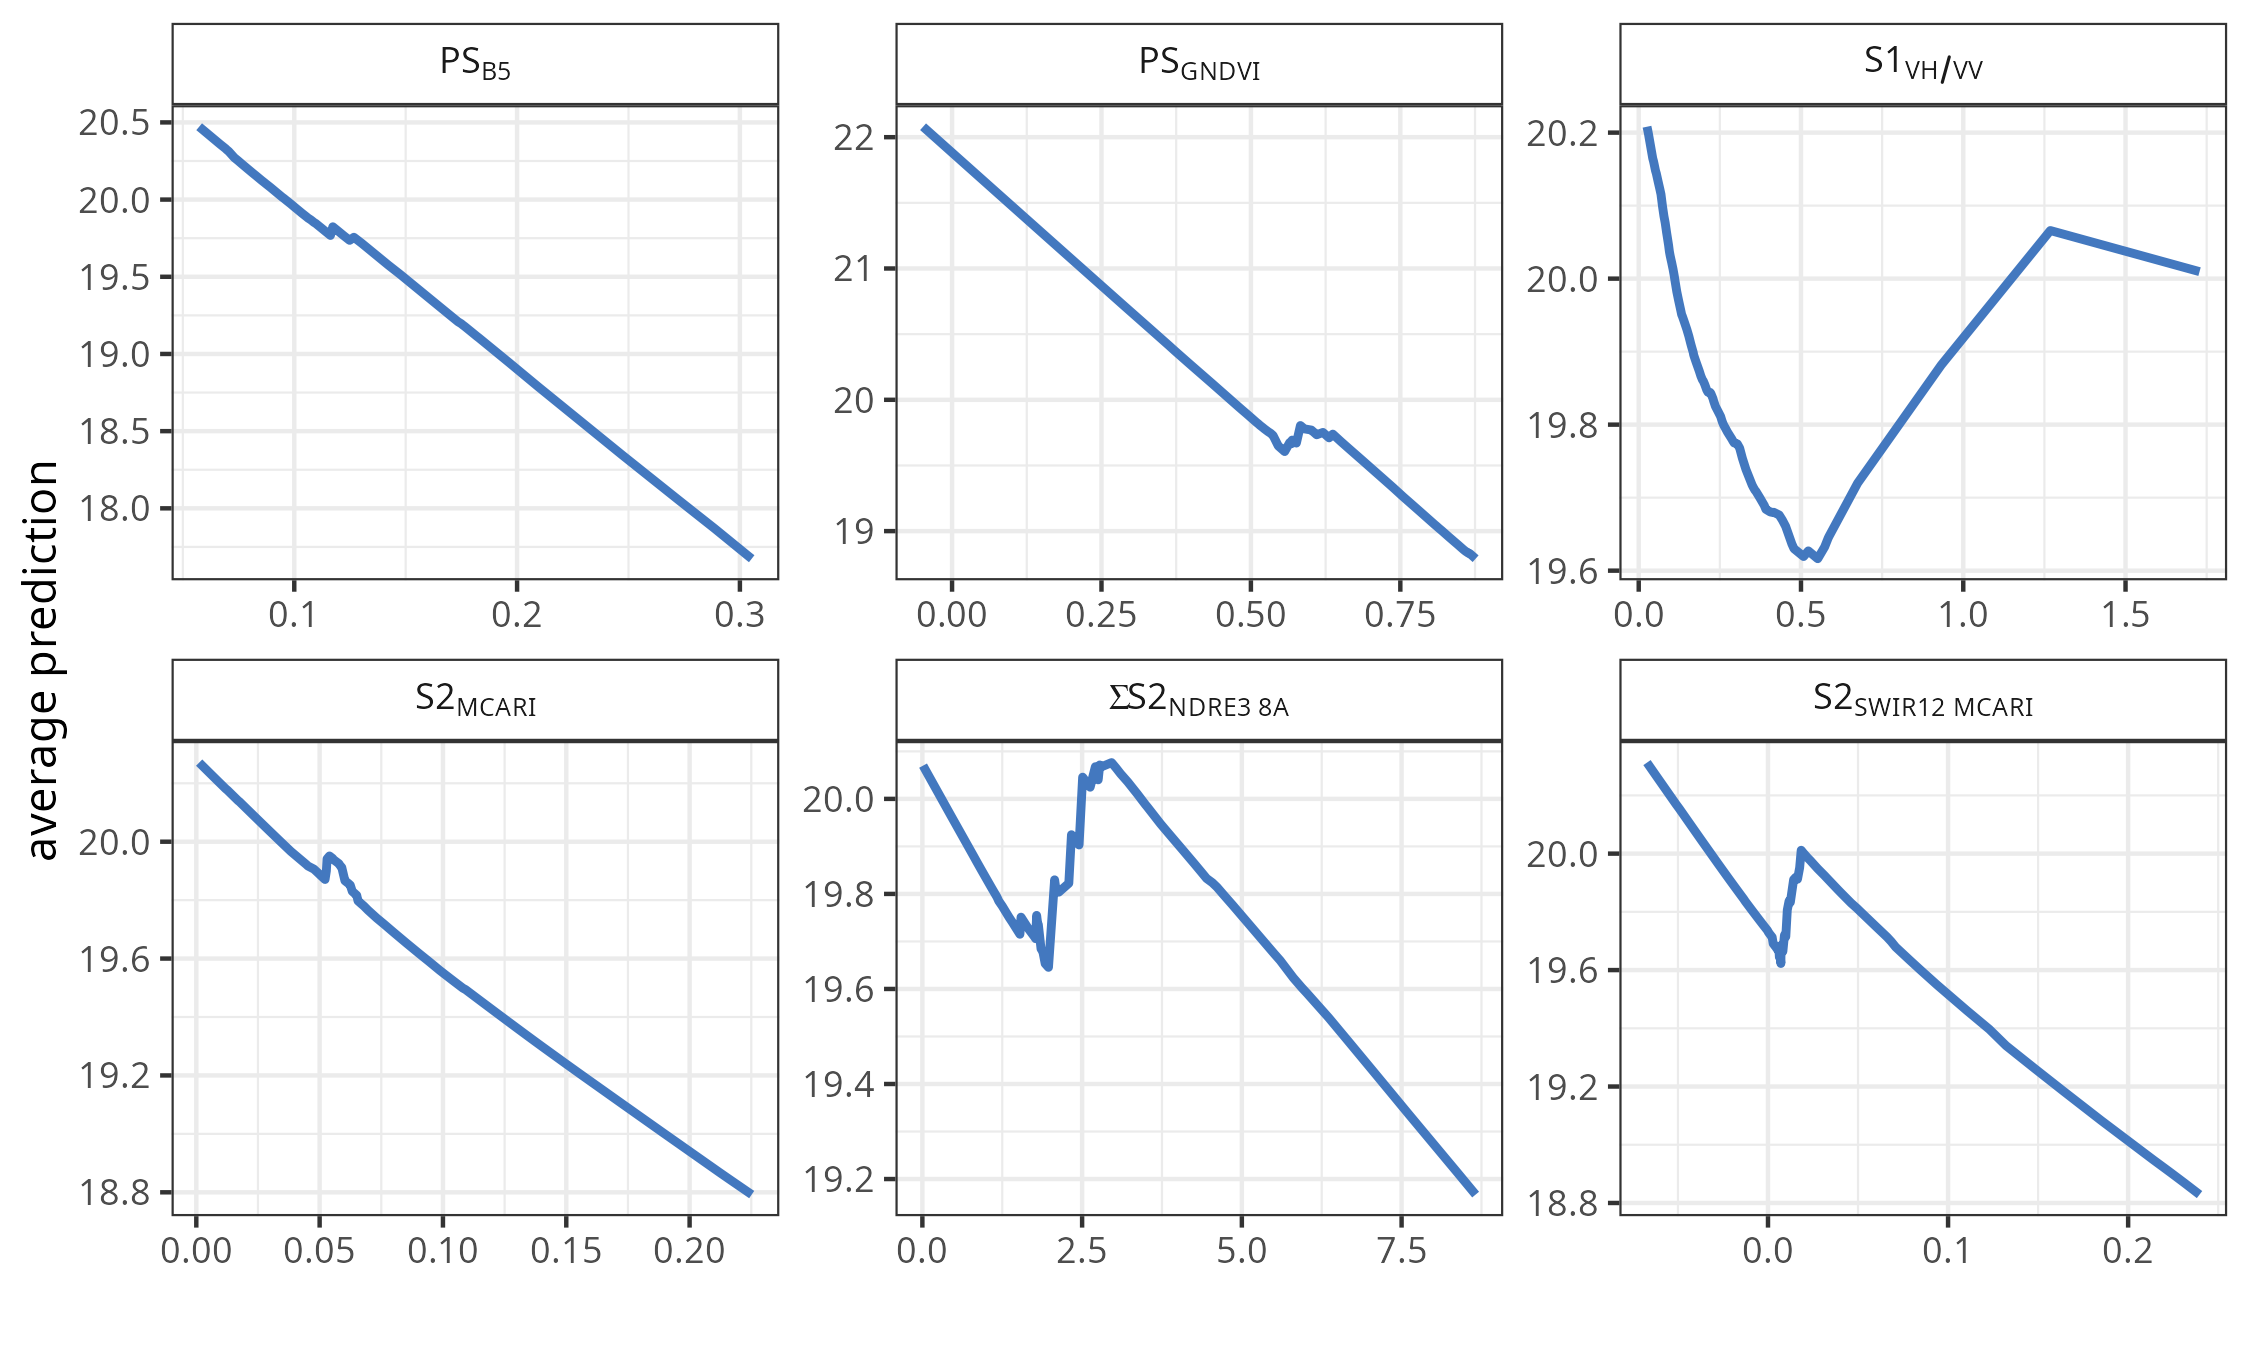
\includegraphics[width=1\linewidth,height=\textheight,keepaspectratio]{../output/figs/partial_dependence_plots_estimation_LOSO.png}

}

\caption{\label{fig-7}\textbf{Partial dependence plots for the six
leading predictors of the LOSO-tuned ensemble model (recipe \emph{rec1},
all predictors).} Each panel shows the average predicted AGB (t/ha,
y-axis) as a function of the predictor value (x-axis), with all other
predictors held at their observed distribution. The ∑ symbol indicates a
cumulative index computed from the start of the growing season.}

\end{figure}%

Partial dependence plots for the six leading predictors of the
LOSO-tuned ensemble (Figure~\ref{fig-7}) reveal predominantly negative,
near-monotonic relationships for the optical predictors: predicted AGB
decreases by roughly 2 t/ha as PS\textsubscript{B5} increases across its
observed range, by a similar margin as PS\textsubscript{GNDVI} increases
from 0 to 0.8, and more gently for S2\textsubscript{MCARI} and
S2\textsubscript{SWIR12\_MCARI}. The cumulative red-edge index
∑S2\textsubscript{NDRE3\_8A} shows a non-monotonic, oscillating profile
with local maxima and minima spanning about 1 t/ha. The Sentinel-1
backscatter ratio S1\textsubscript{VH/VV} displays a shallow U-shape,
with higher predicted AGB at both low (\textasciitilde0) and high
(\textgreater1) ratio values and a minimum around 0.4--0.6. These
patterns should be interpreted with caution: given the narrow, largely
overlapping importance scores in Figure~\ref{fig-6} and the residual
collinearity among the 42 candidate predictors documented in Section
2.3.3, the marginal effect attributed to any single optical index likely
reflects shared variance with co-varying spectral, SAR, and thermal-time
predictors rather than an isolated physiological response. This
collinearity-based caution applies with particular force to the
Sentinel-1 VH/VV ratio: its comparatively high ensemble-level importance
in Figure~\ref{fig-6} reflects variance shared with co-varying optical
and thermal-time predictors, and is therefore not in conflict with the
sensor-ablation result (Table Table~\ref{tbl-6}), in which Sentinel-1
added essentially no marginal skill once those optical and weather
predictors were already present.

\subsubsection{Spatio-temporal variation of AGB within the growing
season}\label{spatio-temporal-variation-of-agb-within-the-growing-season}

Finally, we run the models to make a daily spatial estimation of biomass
through the growing season at each site. The averaged daily AGB for each
site is shown in Figure~\ref{fig-8}, along with the in-situ AGB
measurements.

\begin{figure}

\centering{

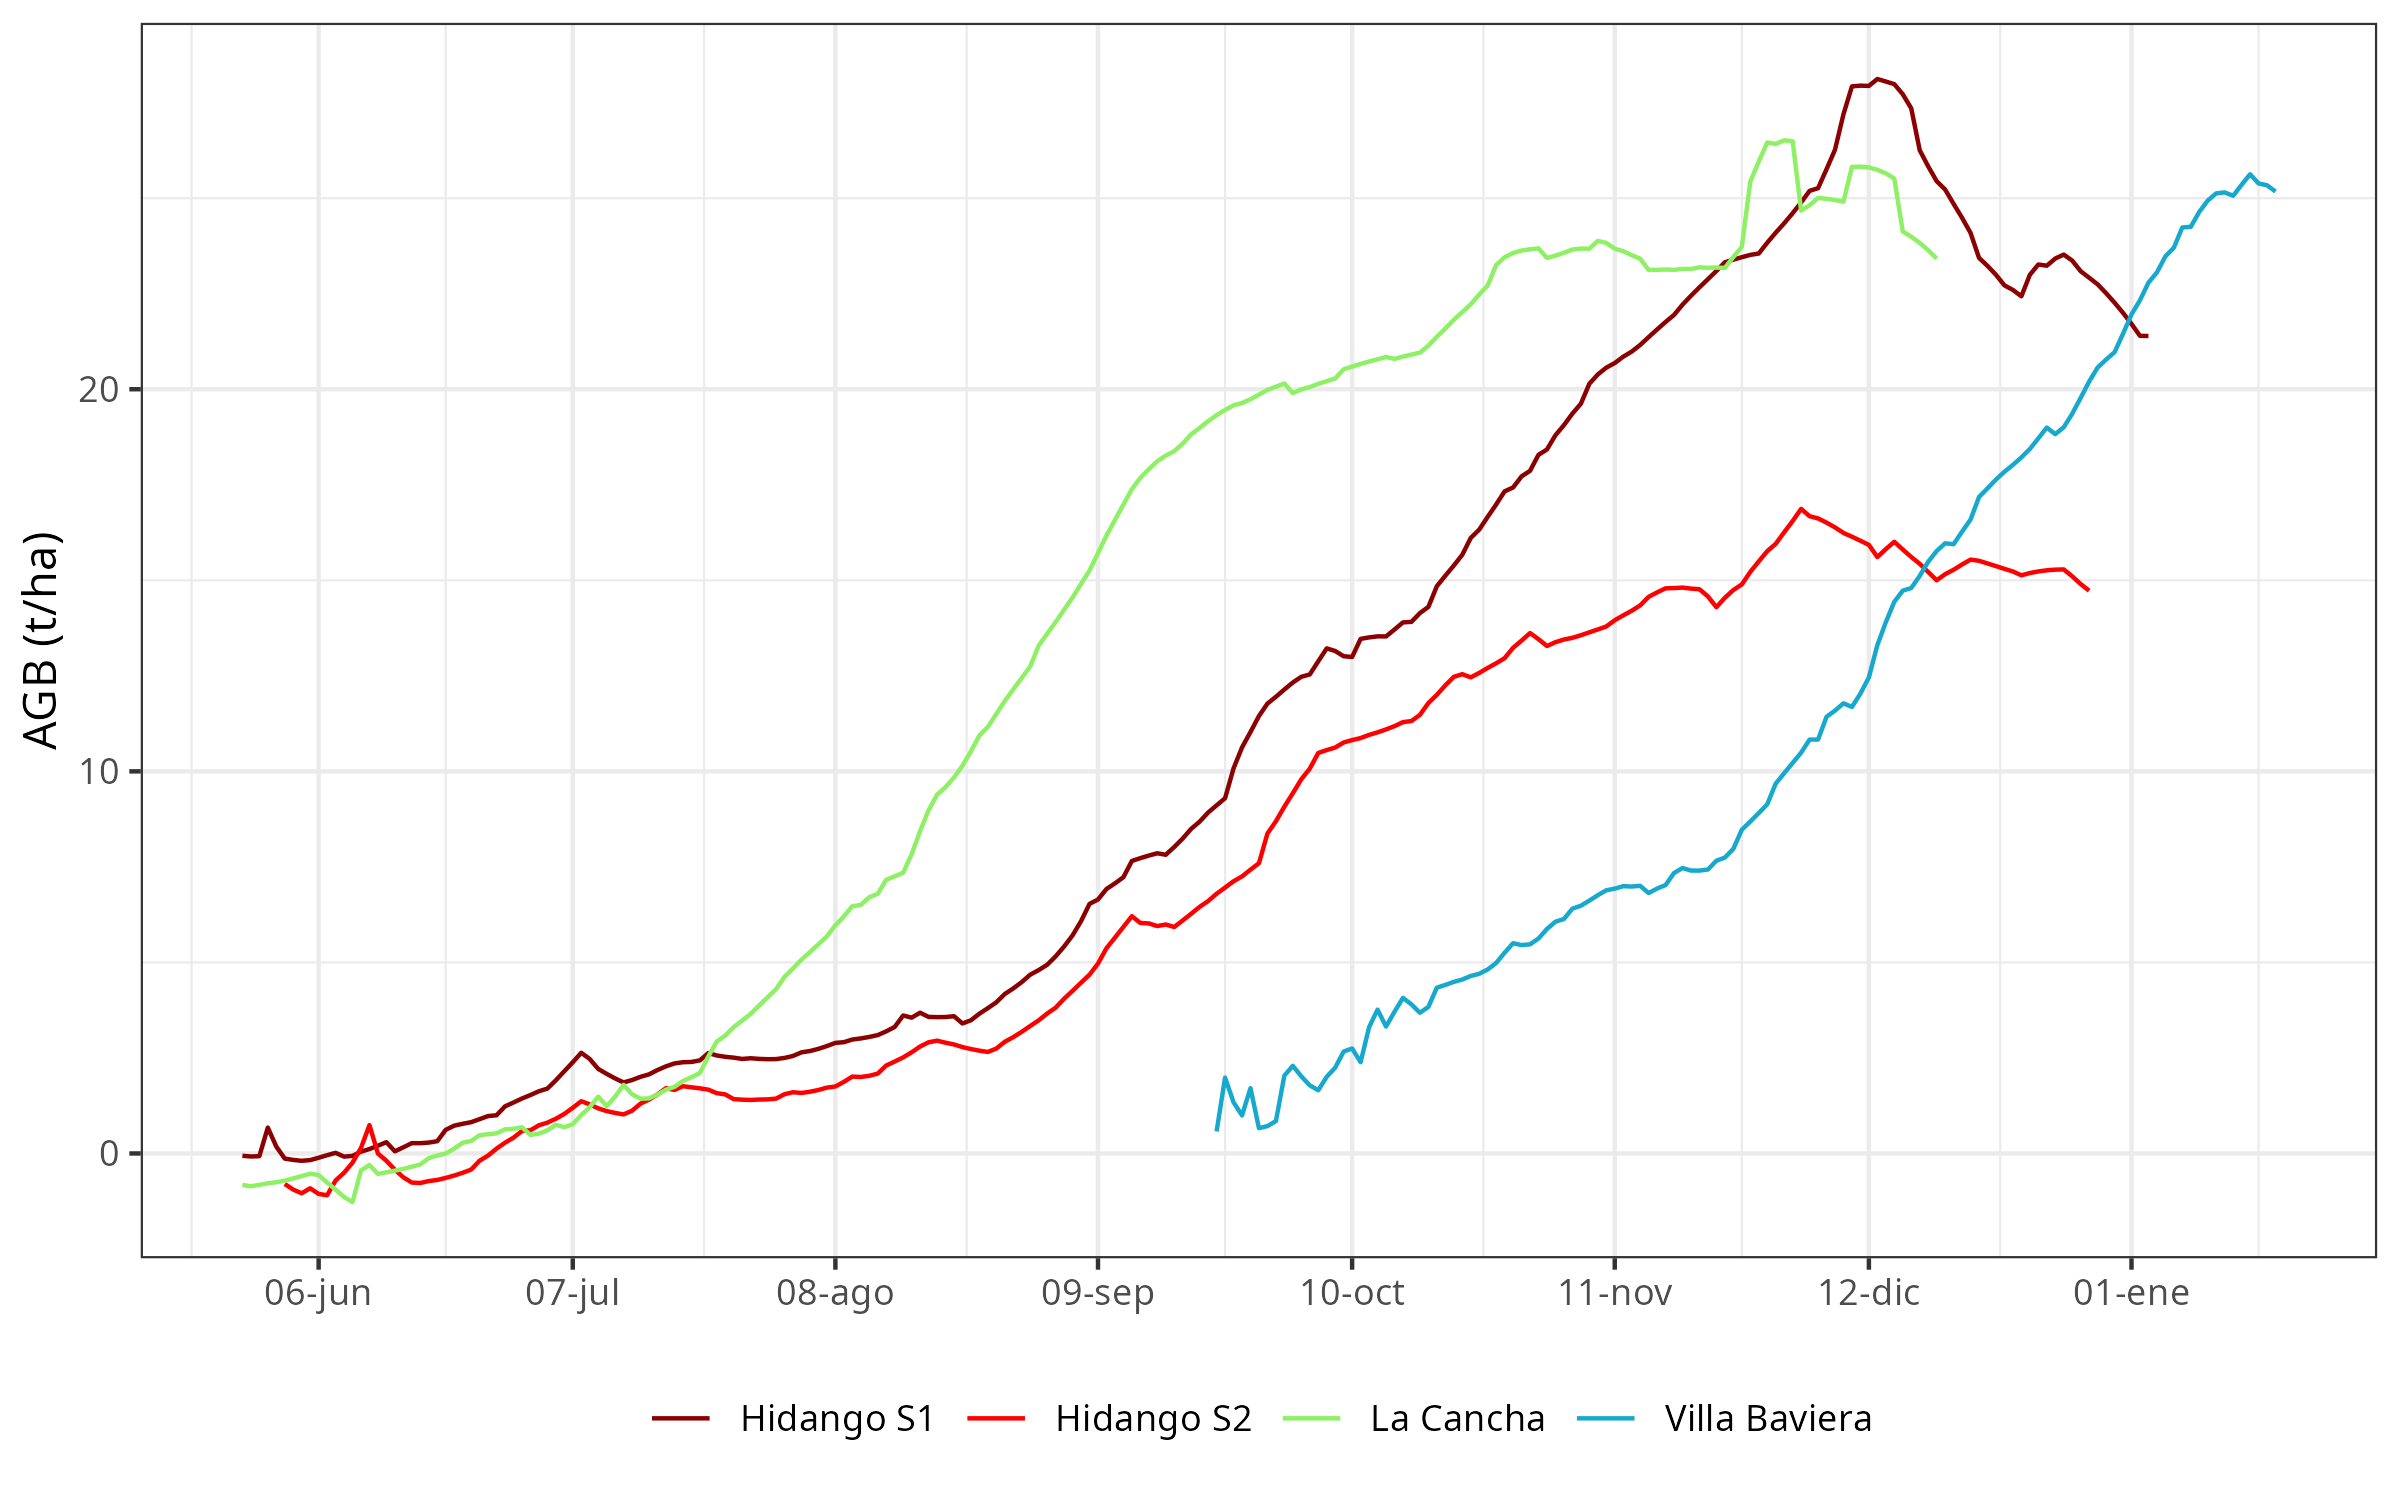
\includegraphics[width=1\linewidth,height=\textheight,keepaspectratio]{../output/figs/time_series_AGB_mean_sites.png}

}

\caption{\label{fig-8}\textbf{Daily temporal variation of the averaged
AGB per site (lines) and the averaged in situ measured AGB per site
(points).} For a better comparison, the dates were turned to the same
year. S1: Season 2021-2022, S2: Season 2022-2023.}

\end{figure}%

The estimation adjusted well for Hidango in both seasons but
underestimated in La Cancha from the middle of the season on. For Villa
Baviera, the model estimates well for most of the season, but at the end
shows an overestimation. In Figure~\ref{fig-9}, we show the monthly
average of AGB per site. In Hidango season 2021-2022 and in La Cancha,
the AGB goes from below 2 t/ha to up to 30 t/ha. In Hidango season
2022-2023, the AGB was lower, reaching 22.50 t/ha. In Villa Baviera, the
wheat variety has a shorter season, from September to January; the AGB
at harvest was up to 30 t/ha. The sites that showed the higher spatial
variability were Hidango season 2022-2023 and La Cancha
(Figure~\ref{fig-8} and Figure~\ref{fig-9}).

\begin{figure}

\centering{

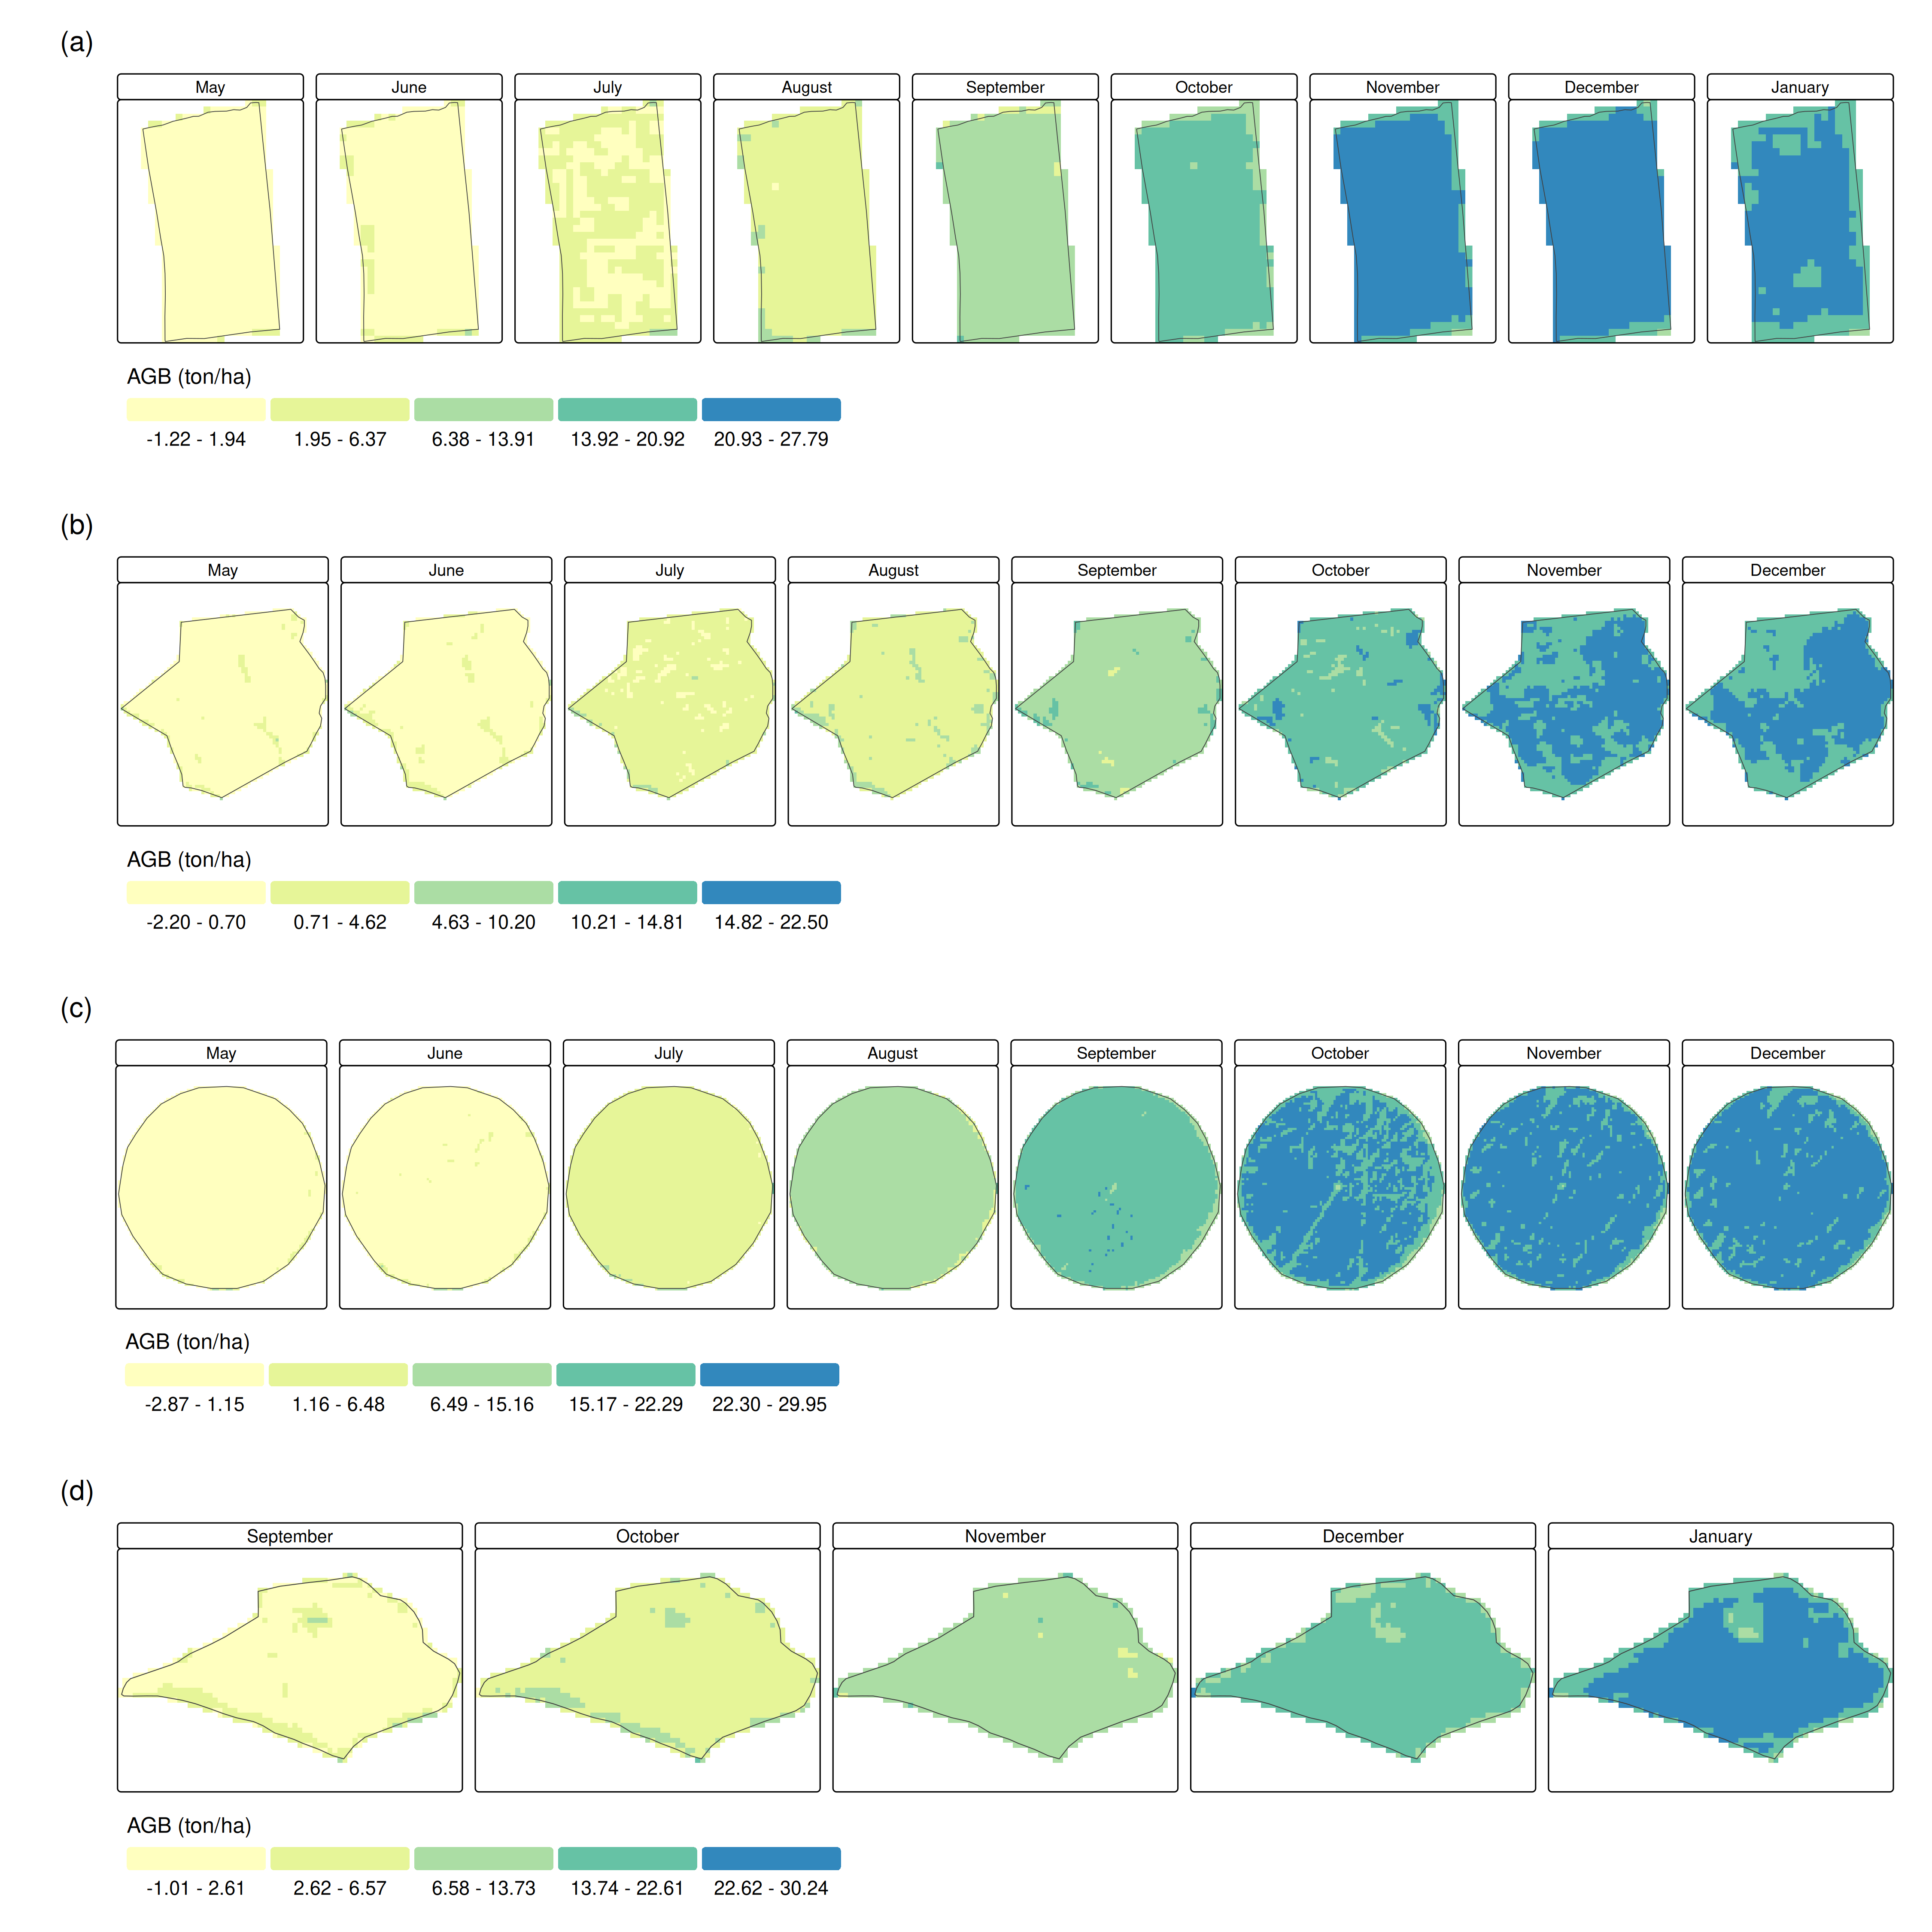
\includegraphics[width=1\linewidth,height=\textheight,keepaspectratio]{../output/figs/mapas_biomasa_mensual_estimada.png}

}

\caption{\label{fig-9}\textbf{Monthly averaged above-ground biomass
(AGB) estimated with the stacked ensemble model (recipe rec1, all
predictors) for the sites} (a) Hidango season 2021-2022, (b) Hidango
season 2022-2023, (c) La Cancha season 2022-2023, and (d) Villa Baviera
season 2020-2021.}

\end{figure}%

\subsection{Prediction models for AGB at
harvest}\label{prediction-models-for-agb-at-harvest-1}

As a secondary, exploratory objective, we used the same
leave-one-site-out cross-validation (LOSO-CV) framework (recipe
\emph{rec1}, all predictors) to evaluate whether covariates available
one to four months before harvest are sufficient to reproduce the stage
1 model's own spatial AGB prediction at the harvest date (Section
2.3.5)---a self-consistency check on the modeling pipeline rather than
validation against independent harvest-date measurements---comparing
four fixed-hyperparameter algorithms (RF, XGBoost, KNN, and bagMLP);
GLMnet was excluded from this comparison because its cross-fold RMSE was
highly unstable (15.5--54.7 t/ha across leads). Random Forest (RF) was
the most consistently competitive of the four across lead times and is
used as the reference model below. For RF, R² decreased from 0.46
(RMSE=4.52 t/ha, MAE=4.21 t/ha) at a one-month lead to 0.25 (RMSE=5.07
t/ha, MAE=4.73 t/ha) at two months, 0.15 (RMSE=5.09 t/ha, MAE=4.73 t/ha)
at three months, and 0.10 (RMSE=6.46 t/ha, MAE=6.13 t/ha) at four months
(Figure~\ref{fig-10}). The other three models followed a broadly similar
declining trend. These results indicate modest, rapidly decaying
self-consistency between early-season covariates and the stage 1 model's
later-season predictions under LOSO-CV, and should not be read as a
direct estimate of skill at forecasting field-measured AGB at harvest.

\begin{figure}

\centering{

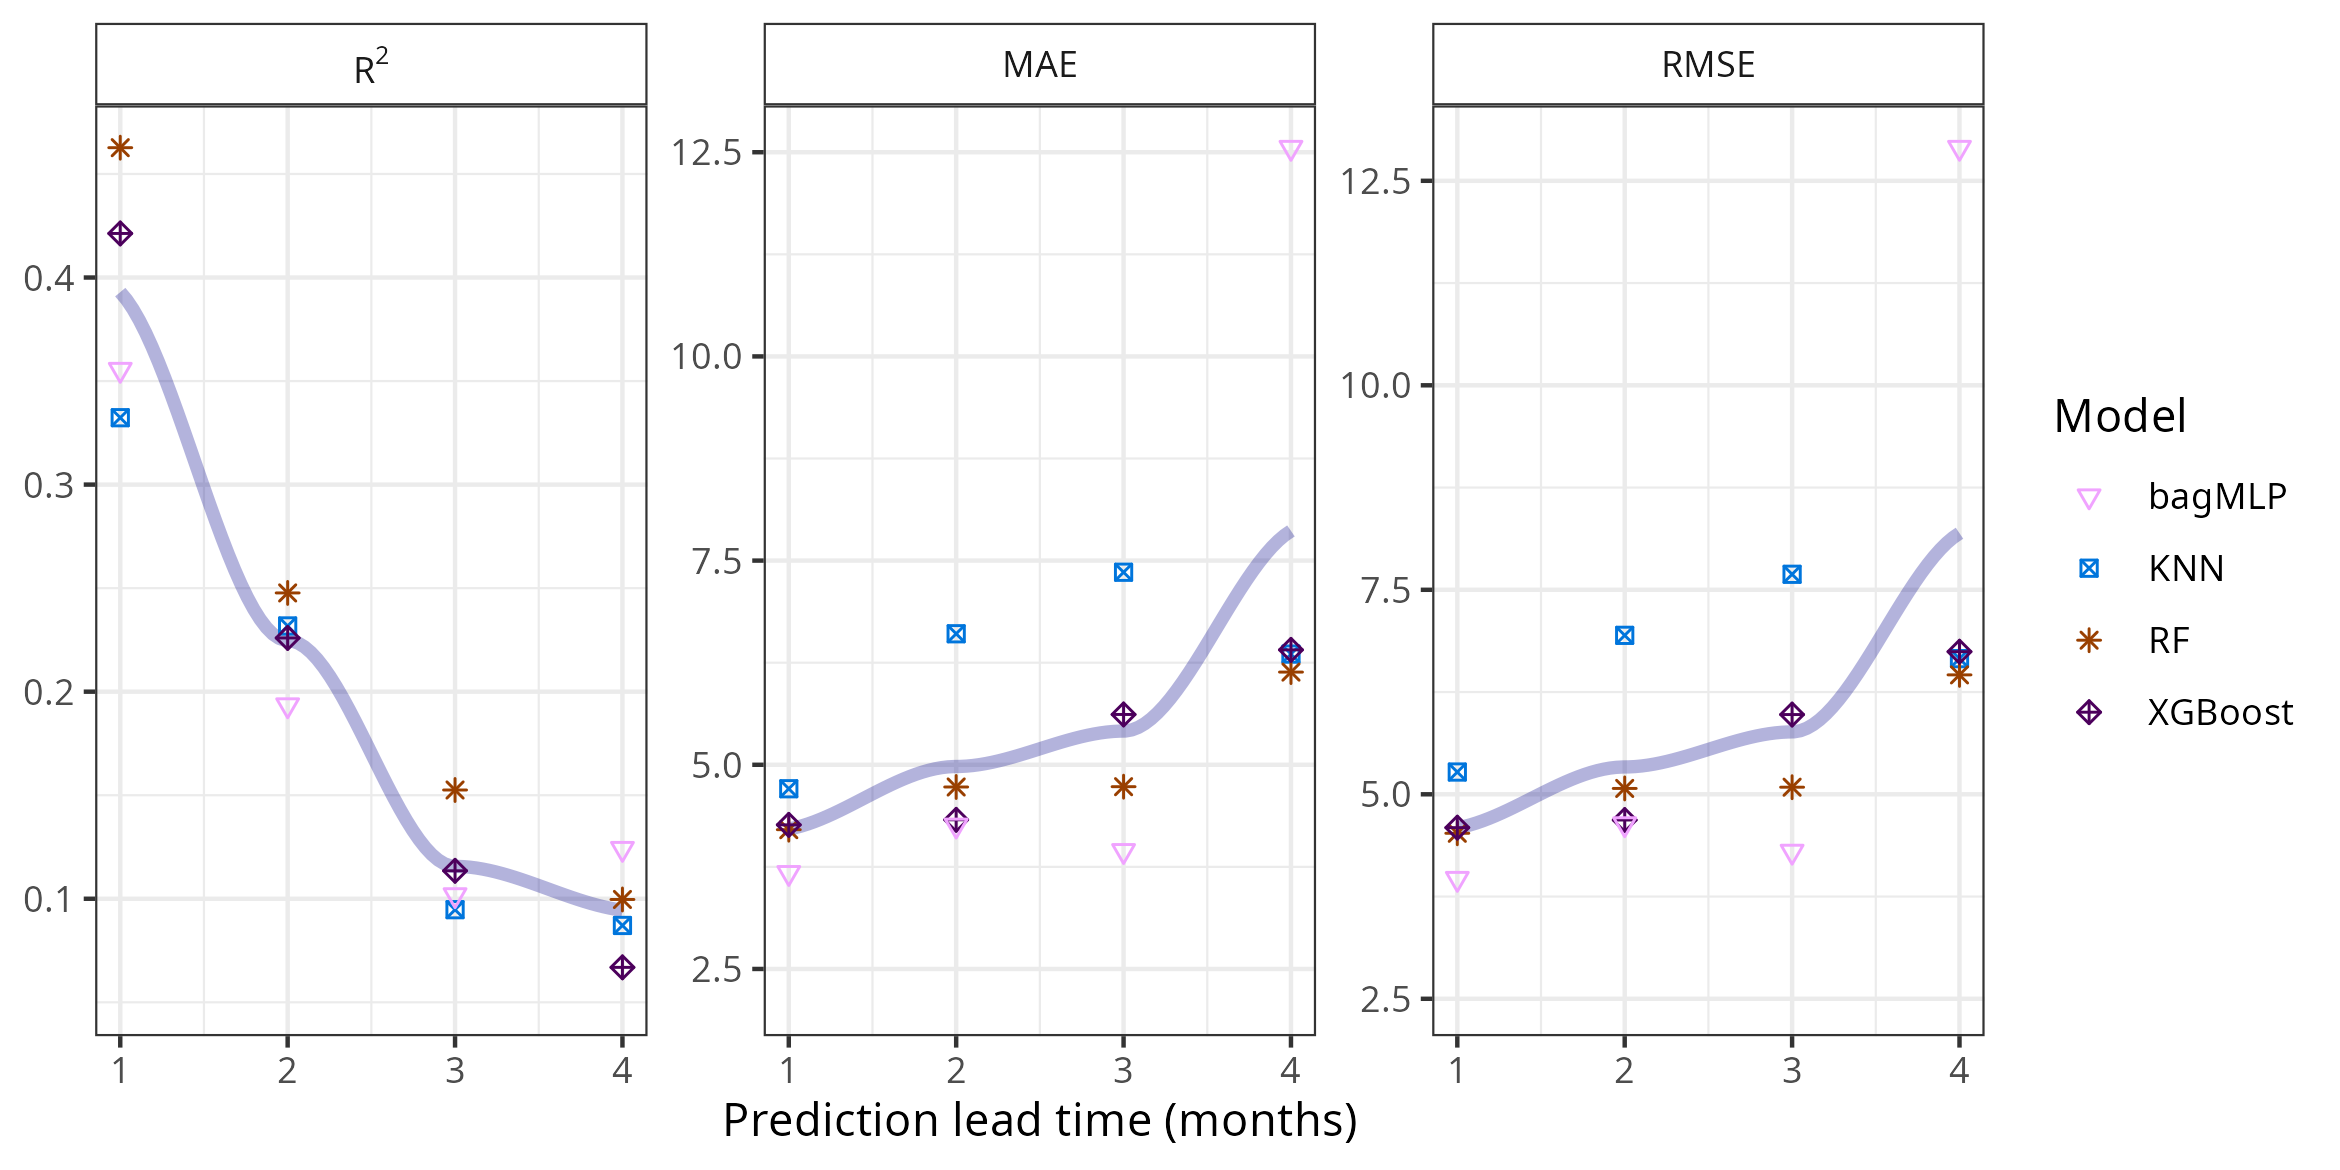
\includegraphics[width=1\linewidth,height=\textheight,keepaspectratio]{../output/figs/metrics_prediction_lead_times.png}

}

\caption{\label{fig-10}\textbf{LOSO-CV performance metrics (R², MAE, and
RMSE, in t/ha) for AGB-at-harvest forecasts one to four months ahead}
(recipe \emph{rec1}, all predictors; best hyperparameter configuration
per fold, as in stage 1), for four fixed-hyperparameter algorithms:
bagged multilayer perceptron (bagMLP), K-nearest neighbors (KNN), random
forest (RF), and extreme gradient boosting (XGBoost). GLMnet was
excluded due to highly unstable cross-fold RMSE (15.5--54.7 t/ha). The
shaded line shows the overall trend (LOESS smooth) across the four
models.}

\end{figure}%

Table~Table~\ref{tbl-5} lists the eight variables with the most
consistent permutation-based importance across the four lead-time RF
models (recipe \emph{rec1}). Soil moisture (SM) had the lowest (best)
overall mean rank (5.75), reflecting its rank-1 importance at the
four-month lead and rank-2/3 importance at the two- and three-month
leads, despite not appearing among the top six predictors at the
one-month lead. By contrast, the cumulative PlanetScope green-red
vegetation index (∑PS\textsubscript{GRVI}) showed a strongly
lead-dependent pattern: it was by far the most important predictor at
one-, two-, and three-month leads (permutation z-scores of 6.2, 4.1, and
4.0, respectively---several times larger than any other variable at
those leads)---but fell to near the bottom of the ranking (42nd of 43
variables) at the four-month lead, yielding a middling overall mean rank
(11.25). The remaining variables in Table~Table~\ref{tbl-5}
(∑S2\textsubscript{B1}, ∑S2\textsubscript{SWIR12\_TCARI},
PS\textsubscript{B8}, S2\textsubscript{NDRE\_NDVI},
PS\textsubscript{B5}, PS\textsubscript{TCARI\_OSAVI}) each appeared
among the top six predictors for at most one or two of the four leads.
Three of these eight variables (∑S2\textsubscript{SWIR12\_TCARI},
PS\textsubscript{B8}, S2\textsubscript{NDRE\_NDVI}) have negative scaled
dropout-loss values, meaning that permuting them slightly reduced,
rather than increased, prediction error on average---a pattern
consistent with noise rather than genuine predictive signal, and a
further indication of the instability discussed below. This pronounced
rotation in variable importance with lead time---with no single
predictor ranking consistently across all four horizons---further
illustrates the instability of harvest forecasting under a
four-site-season LOSO-CV scheme and reinforces the need for larger
multi-site networks to support reliable multi-month forecasting (see
Discussion).

\begin{longtable}[]{@{}
  >{\raggedright\arraybackslash}p{(\linewidth - 8\tabcolsep) * \real{0.1795}}
  >{\raggedright\arraybackslash}p{(\linewidth - 8\tabcolsep) * \real{0.0897}}
  >{\raggedright\arraybackslash}p{(\linewidth - 8\tabcolsep) * \real{0.1923}}
  >{\raggedright\arraybackslash}p{(\linewidth - 8\tabcolsep) * \real{0.2051}}
  >{\raggedright\arraybackslash}p{(\linewidth - 8\tabcolsep) * \real{0.3333}}@{}}
\caption{The eight most important variables (ranked by mean rank) for
the RF prediction model (recipe rec1, all predictors) across the four
LOSO-CV lead-time models. N: number of leads (of four) in which the
variable was among the five most important. Mode rank: most frequent
rank across the four leads. Mean rank: average rank across the four
leads (lower values indicate more consistent importance). Scaled dropout
loss: mean z-scored permutation-importance loss (RMSE increase after
permutation) across the four leads.}\label{tbl-5}\tabularnewline
\toprule\noalign{}
\begin{minipage}[b]{\linewidth}\raggedright
\textbf{Variable}
\end{minipage} & \begin{minipage}[b]{\linewidth}\raggedright
\textbf{N}
\end{minipage} & \begin{minipage}[b]{\linewidth}\raggedright
\textbf{Mode rank}
\end{minipage} & \begin{minipage}[b]{\linewidth}\raggedright
\textbf{Mean rank}
\end{minipage} & \begin{minipage}[b]{\linewidth}\raggedright
\textbf{Scaled dropout loss}
\end{minipage} \\
\midrule\noalign{}
\endfirsthead
\toprule\noalign{}
\begin{minipage}[b]{\linewidth}\raggedright
\textbf{Variable}
\end{minipage} & \begin{minipage}[b]{\linewidth}\raggedright
\textbf{N}
\end{minipage} & \begin{minipage}[b]{\linewidth}\raggedright
\textbf{Mode rank}
\end{minipage} & \begin{minipage}[b]{\linewidth}\raggedright
\textbf{Mean rank}
\end{minipage} & \begin{minipage}[b]{\linewidth}\raggedright
\textbf{Scaled dropout loss}
\end{minipage} \\
\midrule\noalign{}
\endhead
\bottomrule\noalign{}
\endlastfoot
\textbf{SM} & 3 & 1 & 5.75 & 1.91 \\
∑S2\textsubscript{B1} & 2 & 2 & 8.25 & 1.23 \\
∑S2\textsubscript{SWIR12\_TCARI} & 1 & 5 & 9.75 & -0.11 \\
\textbf{∑PS\textsubscript{GRVI}} & 3 & 1 & 11.25 & 3.24 \\
PS\textsubscript{B8} & 0 & 8 & 11.75 & -0.09 \\
S2\textsubscript{NDRE\_NDVI} & 0 & 9 & 12 & -0.12 \\
PS\textsubscript{B5} & 2 & 2 & 12.75 & 0.56 \\
PS\textsubscript{TCARI\_OSAVI} & 3 & 5 & 13 & 0.45 \\
\end{longtable}

\section{Discussion}\label{discussion}

\subsection{Models performance}\label{models-performance}

For in-season AGB estimation, leave-one-site-out cross-validation
(LOSO-CV) across four Mediterranean wheat field-seasons spanning three
locations, two wheat habits (winter and spring), and distinct soil types
offered a preliminary, exploratory assessment of spatial
transferability: because each of the four LOSO folds confounds geography
with soil type and, for the Villa Baviera fold, wheat habit (see Study
limitations below), these results should be read as an indicative
sensitivity analysis rather than as definitive proof of transferability
to new, unseen sites. Under this scheme, the best-performing
configuration (RF using only PlanetScope predictors, recipe \emph{rec7})
reached R²=0.78 (RMSE=7.87 t/ha, MAE=5.90 t/ha); as discussed in Methods
(Section 2.3.6), this and the other LOSO-CV performance estimates may
carry some optimistic bias from the hyperparameter-selection procedure,
so absolute values should be read with appropriate caution while the
relative ranking among recipes and algorithms is more robust. This R² is
broadly comparable to studies that used UAV imagery
\citep{AtkinsonAmorim2022, Liu2024} or hyperspectral data
\citep{Marshall2022} (R²=0.81-0.91), despite the more demanding
cross-site validation applied here, since those studies typically relied
on within-site or random data splits that do not test spatial
transferability. The higher absolute RMSE and MAE relative to those
single-site studies likely reflect the wider AGB range and greater
inter-site/inter-season heterogeneity sampled here (AGB up to
\textasciitilde30 t/ha across winter and spring wheat).

Contrary to our initial expectation that the all-predictors recipe
(\emph{rec1}) or a Sentinel-1-plus-weather combination (\emph{rec3})
would perform best, recipes built on PlanetScope alone (\emph{rec7}) or
with weather (\emph{rec8}) consistently outranked \emph{rec1}, while the
Sentinel-1-only recipe (\emph{rec2}) was consistently among the
worst-performing (R²=0.44-0.53). The complementary sensor-ablation
analysis (Table~Table~\ref{tbl-6}) corroborates this pattern: adding
Sentinel-2 to a weather-only baseline reduced RMSE by 23.4\%, whereas
adding Sentinel-1 to a Sentinel-2-plus-weather model left RMSE
essentially unchanged (+0.5\%), and subsequently adding PlanetScope
produced a further 5.7\% reduction. Under LOSO-CV, therefore, optical
sensors (PlanetScope and Sentinel-2) carry most of the transferable AGB
signal, whereas Sentinel-1 backscatter alone adds little once optical
and weather data are available---a different picture from within-site
evaluations, where SAR-derived indices are often reported among the
strongest predictors \citep{Wang2023}.

At the ensemble level (recipe \emph{rec1}, all predictors),
permutation-based variable importance (Figure~\ref{fig-6}) shows a
comparatively flat ranking: a Sentinel-2 SWIR-related chlorophyll index
(S2\textsubscript{SWIR12\_MCARI}) ranks highest, closely followed by two
PlanetScope predictors (PS\textsubscript{B5}, PS\textsubscript{GNDVI}),
a cumulative Sentinel-2 red-edge index (∑S2\textsubscript{NDRE3\_8A}),
S2\textsubscript{MCARI}, the Sentinel-1 VH/VV ratio, ∑GDD,
S1\textsubscript{VH}, S2\textsubscript{B1}, and
S2\textsubscript{MCARI\_OSAVI2}---all within a narrow range of
dropout-loss values. This indicates that, once combined in a single
model, optical, SAR, and accumulated thermal-time predictors carry
comparable, partly redundant information, consistent with the residual
collinearity documented by the VIF audit (Section 2.3.3). The partial
dependence profiles for these leading predictors (Figure~\ref{fig-7})
are predominantly negative and, for the Sentinel-1 VH/VV ratio,
non-monotonic (U-shaped); given this collinearity, we interpret these
marginal effects with caution rather than as isolated physiological
responses.

For the secondary, exploratory objective (stage 2), the same LOSO-CV
scheme applied to the 1-4-month lead-time dataset (recipe \emph{rec1},
RF as the most stable model across leads) yielded modest and rapidly
decaying self-consistency between early-season covariates and the stage
1 model's harvest-date prediction: R² fell from 0.46 (RMSE=4.52 t/ha) at
one month to 0.10 (RMSE=6.46 t/ha) at four months. Permutation
importance for these RF models (Table~Table~\ref{tbl-5}) showed a
pronounced rotation across lead times rather than a stable set of top
predictors: the cumulative PlanetScope green-red index
(∑PS\textsubscript{GRVI}) dominated at one-, two-, and three-month leads
but became unimportant at four months, while soil moisture (SM) became
the leading predictor only at the four-month lead. This instability,
together with the modest and rapidly decaying R², is consistent with the
limited number of independent site-seasons (n=4) available to a
leave-one-site-out scheme: each fold trains on only three site-seasons
and is evaluated on a fourth, entirely unseen field, season, and (in
most folds) wheat habit. Beyond this small-sample instability, a more
fundamental limitation is that the stage 2 target is itself a stage 1
model output rather than an independent harvest-AGB ground truth
(Section 2.3.5): even with a larger network of site-seasons, this design
would remain a test of internal consistency between early- and
late-season model behavior rather than of true forecasting skill against
field-measured biomass. We therefore interpret these results as a proof
of concept for the modeling pipeline rather than as evidence of
operational forecasting skill, and as a call for both larger multi-site,
multi-season networks and an independent harvest-date sampling campaign
to properly evaluate multi-month AGB forecasting (see Study
limitations).

\subsection{Application for wheat yield
management}\label{application-for-wheat-yield-management}

The ability to estimate in-season AGB with policy-relevant accuracy
(\emph{rec7}\_RF, R²=0.78) can support irrigation, fertilization, and
crop-insurance decisions, as well as yield monitoring by government
agencies. However, our sensor-ablation results temper one common
assumption in the literature: under LOSO-CV, Sentinel-1 backscatter did
not improve on an optical-plus-weather baseline (+0.5\% RMSE), so SAR
should not be regarded as a source of additional accuracy when optical
imagery is available. Its practical value is more likely as a substitute
rather than a complement: maintaining partial model coverage during
persistent cloud cover, when Sentinel-2 or PlanetScope observations are
unavailable. Confirming this cloud-substitution role, and quantifying
any accuracy trade-off relative to a fully-optical pipeline, would
require evaluating model performance under simulated optical data
gaps---an analysis beyond the scope of the present study but a natural
direction for future work.

In contrast to UAV- or hyperspectral-based approaches, this framework
offers lower equipment and operational costs. The best-performing
configuration (\emph{rec7}\_RF) relies on PlanetScope imagery without
requiring in-situ soil moisture, and a fully public alternative
(Sentinel-2 plus weather, \emph{rec6}) captures a substantial share of
the achievable improvement (a 23.4\% RMSE reduction over a weather-only
baseline). This suggests two complementary deployment pathways: a fully
public Sentinel-2-plus-weather pipeline that is, in principle,
transferable to any region with public meteorological data, and a
higher-accuracy PlanetScope-based pipeline that requires a commercial
imagery subscription. In both cases, however, the framework's reliance
on in-situ weather station data (discussed below) remains the main
barrier to low-cost, large-scale deployment, and the LOSO-CV results
indicate that performance at new, unmonitored sites would still need to
be validated before operational use.

To place the stage 2 forecasting numbers in a decision-making context:
at a one-month lead, an RMSE of 4.5 t/ha on AGB values reaching up to
\textasciitilde30 t/ha corresponds to a relative error of roughly 15\%,
which could support farm-level triage decisions---for example, flagging
fields tracking substantially below their expected biomass trajectory
for closer monitoring, supplemental irrigation, or adjusted
fertilization timing---but would likely be too coarse for fine-grained
input allocation (e.g., variable-rate fertilization) or for
individual-field crop-insurance payouts, which typically require errors
below \textasciitilde10\%. By four months, the near-zero R² (0.10) and
RMSE of 6.5 t/ha indicate that field-level forecasts are not yet
reliable enough to inform individual management decisions at this
horizon; at that stage, the framework's value would be limited to
regional-scale aggregation, where individual-field errors partly average
out, supporting early-warning systems for below-average regional yields
rather than field-specific actions.

\subsection{Study limitations}\label{study-limitations}

The weather data used here come from stations within or near the study
fields. Regional or fully scalable applications would need to evaluate
performance using satellite-derived weather products (e.g., CHIRPS,
ERA5). Soil moisture (SM) measurements, used as a predictor, require
dedicated in-field sensors that many farmers and monitoring programs
lack; while SM was not among the leading predictors for in-season
estimation (stage 1), it emerged as the most important predictor for
four-month-ahead forecasting (stage 2, Table~Table~\ref{tbl-5}), so its
availability remains relevant for longer-horizon applications. Advances
in satellite-based soil moisture estimation at the farm scale
\citep{VanHateren2023, Zeyliger2022} could help address this dependence
and facilitate generalization.

Another limitation is that this study is based on three locations (four
site-seasons) in central Chile, covering winter and spring wheat
varieties. The leave-one-site-out cross-validation scheme used
throughout this study is, by design, a conservative estimate of
transferability to new sites, but with only four site-seasons each LOSO
fold trains on just three of them---particularly limiting for the stage
2 forecasting models, where the rotation in variable importance across
lead times (Table~Table~\ref{tbl-5}) likely reflects this small sample
as much as genuine seasonal dynamics. Expanding the AGB dataset to more
sites, seasons, and varieties is the most direct way to improve and
properly evaluate generalization; however, in Chile, reliable and
publicly available farm-scale wheat AGB data remain scarce.

A further methodological limitation concerns the
hyperparameter-selection procedure described in Section 2.3.6: because
the held-out LOSO fold is used both to select the best hyperparameter
configuration and to report its performance, the reported R², RMSE, and
MAE values---including the headline \emph{rec7}\_RF estimate,
R²=0.78---may be optimistically biased relative to a fully nested
cross-validation, in which hyperparameter tuning would be confined to
the training folds only. We were unable to implement a nested LOSO-CV
here because, with only four site-seasons, an inner-loop split would
leave too few independent units per fold to tune hyperparameters
meaningfully. The fixed-hyperparameter sensor-ablation analysis (Table
Table~\ref{tbl-6}), which is not subject to this issue, corroborates the
recipe-level ranking and the near-zero marginal contribution of
Sentinel-1, suggesting that the qualitative, relative conclusions of
this study are more robust than the absolute performance values. We
recommend that studies with a larger number of site-seasons implement
nested cross-validation, confining hyperparameter selection strictly to
training data, to obtain unbiased generalization-error estimates.

A related limitation is that the experimental design confounds wheat
habit with location: Villa Baviera is the only spring-wheat site-season,
while the other three are winter wheat. As a result, the LOSO fold in
which Villa Baviera is held out simultaneously tests transferability to
a new location, a new soil type, and a different wheat habit, so it is
not possible to fully disentangle whether model performance and the
variable-importance patterns reported here reflect generalizable wheat
phenology or site-specific (including habit-specific) effects. Given
this extreme confounding in a four-fold design, we emphasize that the
LOSO-CV results reported throughout this study---including the headline
R²=0.78 for the \emph{rec7}\_RF configuration---constitute a preliminary
sensitivity analysis of spatial transferability rather than a definitive
demonstration that the framework generalizes to new sites, soils, or
wheat habits. Resolving this confound would require additional
spring-wheat site-seasons at locations other than Villa Baviera, which
we identify as a priority for future data collection.

A further limitation specific to the secondary, exploratory forecasting
objective (stage 2, Section 2.3.5) is that its response variable is the
stage 1 model's own spatial prediction at the harvest date rather than
an independent, field-measured AGB value. The stage 2 results (Section
3.2) therefore demonstrate the internal consistency of the modeling
pipeline---i.e., the extent to which pre-harvest covariates can
reproduce the stage 1 model's later-season output---but do not
constitute evidence that the framework can forecast actual,
field-measured biomass at harvest; a genuine test of forecasting skill
would require a dedicated destructive-sampling campaign at the harvest
date, independent of the stage 1 model. Relatedly, the 100 samples per
site-season used for stage 2 modeling are drawn from a smoothed,
spatially-autocorrelated stage 1 prediction surface rather than from
independent biological replicates, so the nominal sample size (400
across four site-seasons) overstates the effective, independent
information content of the stage 2 dataset and may understate the true
uncertainty of the reported stage 2 metrics. We therefore present the
stage 2 results strictly as an exploratory proof of concept, and
recommend that future work pair this modeling framework with independent
in-situ harvest-AGB measurements before drawing conclusions about
real-world forecasting performance.

Other concerns include the speckle noise inherent to Sentinel-1 and its
dependence on incidence angle, which may have contributed to its limited
marginal contribution under LOSO-CV (Table~Table~\ref{tbl-6}) and could
make consistent SAR-based performance across landscapes or farming
systems challenging. Finally, the residual collinearity among cumulative
vegetation indices, documented by the VIF audit (Section 2.3.3), affects
not only the flat ensemble-level variable importance
(Figure~\ref{fig-6}) but the reliability of permutation-based importance
itself (Section 2.3.3): because permuting one of several correlated
predictors generates unrealistic, out-of-distribution combinations, the
rankings in Figure~\ref{fig-6} and Table Table~\ref{tbl-5} should be
read as identifying groups of mutually-informative predictors rather
than precisely localized individual importances. Future work should
re-run the explainability analysis on the VIF-reduced 22-variable set
identified here, or apply conditional permutation importance methods
designed for correlated predictors, before drawing fine-grained
conclusions about individual variable contributions.

\section{Conclusion}\label{conclusion}

In this study, we evaluated 40 recipe-algorithm combinations---eight
sensor-combination recipes (weather, Sentinel-1, Sentinel-2, and
PlanetScope, individually and combined) and five ML algorithms---plus a
stacked ensemble, to estimate in-season wheat AGB (stage 1) under a
preliminary leave-one-site-out spatial cross-validation across four
Mediterranean field-seasons (see Discussion, Study limitations, for
caveats regarding the confounding of geography with wheat habit and the
hyperparameter-selection procedure). The best-performing model used only
PlanetScope predictors with Random Forest (\emph{rec7}\_RF, R²=0.78,
RMSE=7.87 t/ha, MAE=5.90 t/ha); RF and XGBoost were generally the
strongest algorithms, while the all-predictors recipe (\emph{rec1}) and
the Sentinel-1-only recipe (\emph{rec2}) ranked lower. A sensor-ablation
analysis confirmed that optical sensors (Sentinel-2, PlanetScope) drive
most of the transferable AGB signal, while Sentinel-1 backscatter adds
essentially no skill once optical and weather data are available. At the
ensemble level, permutation-based variable importance showed a
comparatively flat ranking among Sentinel-2 and PlanetScope spectral
indices, the Sentinel-1 VH/VV ratio, and accumulated growing degree
days, indicating substantial redundancy among the candidate predictors.

As a secondary, exploratory objective, we used the same LOSO-CV
framework to test, as a self-consistency check, whether covariates
available one to four months before harvest can reproduce the stage 1
model's own spatial AGB prediction at harvest (stage 2, recipe
\emph{rec1}, Random Forest as the most stable algorithm across leads).
Self-consistency was modest and decayed sharply with lead time, from
R²=0.46 (RMSE=4.52 t/ha) at one month to R²=0.10 (RMSE=6.46 t/ha) at
four months, and the leading predictors rotated substantially across
leads---a cumulative PlanetScope green-red index dominated at one to
three months, while soil moisture became most important only at four
months. This decay and instability reflect the limited number of
independent site-seasons (n=4) available to a leave-one-site-out scheme
and underscore that robust multi-month AGB forecasting will require
substantially larger multi-site, multi-season networks. Because the
stage 2 target is itself a stage 1 model output rather than an
independent harvest-AGB measurement, these results demonstrate the
internal consistency of the modeling pipeline rather than validated
forecasting skill against ground truth; independent harvest-date
sampling is needed to establish the latter.

Overall, these results show that an explainable, multi-sensor ML
framework can estimate in-season wheat AGB with policy-relevant
accuracy, with optical sensors (PlanetScope, Sentinel-2) as the primary
drivers of skill and Sentinel-1 offering, at most, a complementary role
under persistent cloud cover; however, given the four-site-season
design, these LOSO-CV results should be regarded as a preliminary
sensitivity analysis rather than definitive proof of generalizability to
new sites, soils, and wheat habits (see Discussion). Harvest forecasting
at multi-month leads remains an open challenge that will benefit from
larger and more diverse site networks. Future work should focus on (i)
expanding the AGB dataset across more sites, seasons, and wheat
varieties---including additional spring-wheat site-seasons---to enable
robust multi-month forecasting and to disentangle geography from wheat
habit in transferability assessments; (ii) testing satellite-derived
weather and soil moisture products (e.g., ERA5, CHIRPS, SAR-based SM) to
reduce dependence on in-situ stations; (iii) re-running the
explainability analysis on the VIF-reduced predictor set or using
conditional permutation importance to address residual collinearity;
(iv) implementing nested cross-validation for hyperparameter selection
as the number of site-seasons grows; and (v) collecting independent
in-situ AGB measurements at harvest to validate the stage 2 forecasting
framework against ground truth rather than against the stage 1 model's
own predictions.

\section{Acknowledgements}\label{acknowledgements}

We thank Dr.~Christian Alfaro from the Instituto de Investigaciones
Agropecuarias (INIA) for his support and for providing access to the
wheat fields. We also thank Professor Francisco Tapia from Universidad
Mayor for his support and his knowledge about wheat development during
this research. Finally, we thank Mr.~Fabian Llanos, who coordinated the
field trips that allowed us to collect the wheat biomass in-situ data.

\section{Data and code availability}\label{data-and-code-availability}

The data and code used for the analysis and modeling of above-ground
biomass (AGB) in wheat fields is openly available at the following
GitHub repository:
\url{https://github.com/FONDECYT-11190360/AGB_wheat_modelling}. This
repository contains data, R scripts and documentation for data
preprocessing, model development, variable importance analysis, and
visualization.

\section{CRediT authorship contribution
statement}\label{credit-authorship-contribution-statement}

\textbf{Francisco Zambrano}: Project administration, Funding
acquisition, Formal analysis, Conceptualization, Methodology, Writing -
Original Draft, Writing - Review \& Editing, Visualization. \textbf{Abel
Herrera}: Formal Analysis, Data curation, Visualization, Writing -
Original Draft, Writing - Review \& Editing. \textbf{Mauricio
Molina-Rocco:} Conceptualization, Writing - Original Draft, Writing -
Review \& Editing.

\section{Declaration of competing
interest}\label{declaration-of-competing-interest}

The authors declare that they have no known competing financial
interests or personal relationships that could have appeared to
influence the work reported in this paper.

\section{Funding Sources}\label{funding-sources}

Chile's National Research and Development Agency (ANID) funded this
study through the grants Fondecyt de Iniciación N°11190360, FONDEF IdEA
I+D ID21I10297, and the drought emergency FSEQ210022. We also like to
thank the Instituto de Investigaciones Agropecuarias (INIA), the
enterprises Ariztia, and Villa Baviera for giving access to the fields
of wheat.

\section{Declaration of generative AI and AI-assisted technologies in
the writing
process}\label{declaration-of-generative-ai-and-ai-assisted-technologies-in-the-writing-process}

During the preparation of this work, the authors used ChatGPT-3.5 and
Microsoft Copilot to polish the writing of the manuscript. After using
this service, the authors reviewed and edited the content as needed and
took full responsibility for the publication.

\section{Glossary}\label{glossary}

\begin{longtable}[]{@{}
  >{\raggedright\arraybackslash}p{(\linewidth - 2\tabcolsep) * \real{0.6098}}
  >{\raggedright\arraybackslash}p{(\linewidth - 2\tabcolsep) * \real{0.3902}}@{}}
\toprule\noalign{}
\begin{minipage}[b]{\linewidth}\raggedright
\textbf{Abbreviation / Term}
\end{minipage} & \begin{minipage}[b]{\linewidth}\raggedright
\textbf{Definition}
\end{minipage} \\
\midrule\noalign{}
\endhead
\bottomrule\noalign{}
\endlastfoot
AGB & Above-Ground Biomass. The total mass of living plant material
(excluding roots) in a given area, typically measured in tons per
hectare (t/ha). It is the primary dependent variable being modeled and
forecasted. \\
ML & Machine Learning. A subset of artificial intelligence that provides
systems with the ability to automatically learn and improve from
experience without being explicitly programmed. \\
SAR & Synthetic Aperture Radar. A type of radar used in satellite remote
sensing (e.g., Sentinel-1) that transmits microwaves and records the
backscattered signal, providing data related to surface roughness and
moisture, independent of weather and light conditions. \\
S1 & Sentinel-1. The European Space Agency (ESA) satellite mission
providing C-band Synthetic Aperture Radar (SAR) data. Used for
monitoring land and ocean surface dynamics. \\
S2 & Sentinel-2. The European Space Agency (ESA) satellite mission
providing high-resolution optical imagery (13 spectral bands). Used for
land cover classification and vegetation monitoring. \\
PlanetScope & A constellation of Earth-observing satellites operated by
Planet Labs. They provide daily, high-resolution optical imagery,
complementing the temporal resolution of Sentinel missions. \\
In-Situ Data & Data collected directly at the field location, involving
physical measurement. In this study, this primarily refers to collected
weather variables and soil moisture measurements. \\
GDD & Growing Degree Days. A measure of heat accumulation used to
predict the rate of plant development between growing stages
(phenological stages). It is calculated based on daily maximum and
minimum air temperatures. \\
SM & Soil Moisture. The water content of the soil, measured here with
TEROS 12 capacitance sensors and used as both a predictor of crop
development and an indicator of water stress. \\
RF & Random Forest. An ensemble learning method that builds multiple
decision trees on bootstrapped samples and averages their predictions,
widely used for its robustness and resistance to overfitting. \\
XGBoost & eXtreme Gradient Boosting. A highly optimized and efficient
open-source implementation of the gradient boosting framework, popular
for its speed and performance in structured data prediction. \\
GLMnet & Generalized Linear Model with regularization. A model that
applies regularized regression (L1/L2 penalties) to linear models, often
used for variable selection and preventing overfitting. \\
KNN & k-Nearest Neighbors. A non-parametric supervised learning method
used for classification and regression. The output is based on the
classification or mean value of its nearest neighbors. \\
bagMLP & Bagged Multilayer Perceptron. An ensemble learning technique
where multiple Multilayer Perceptron (neural network) models are trained
on different subsets of the data (bagging), and their predictions are
averaged. \\
Cross-Validation & A statistical technique used to estimate how
accurately a predictive model will perform in practice. It involves
partitioning the data into subsets for training and testing. \\
LOSO-CV & Leave-One-Site-Out Cross-Validation. A spatial
cross-validation scheme in which each fold corresponds to one entire
site-season; models are trained on the remaining site-seasons and
evaluated on the held-out one, directly testing spatial
transferability. \\
VIF & Variance Inflation Factor. A diagnostic statistic that quantifies
the degree of multicollinearity among predictor variables in a
regression model; values above 10 are commonly considered indicative of
problematic collinearity. \\
R² & Coefficient of Determination. A statistical measure representing
the proportion of the variance for a dependent variable that is
explained by the independent variables in a regression model. A value
closer to 1 indicates a better fit. \\
RMSE & Root Mean Square Error. A measure of the average magnitude of the
errors. It tells you how concentrated the data is around the line of
best fit. It has the same units as the dependent variable (t/ha). \\
MAE & Mean Absolute Error. The average of the absolute differences
between predicted and observed values, expressed in the same units as
the dependent variable (t/ha). Less sensitive to large outliers than
RMSE. \\
DALEX & moDel Agnostic Language for Exploration and eXplanation. A
specific framework or library used in this research to provide
model-agnostic tools for explaining the behavior of complex ML models
(contributing to XAI). \\
\end{longtable}


\bibliography{references.bib}



\end{document}
